\section{Simulation Results}
\label{sec-simulations}

We have implemented the Firefly algorithm in
TinyOS~\cite{tinyos-asplos00} using the TOSSIM~\cite{tossim} simulator
environment. This simulator has several limitations.  It does not
model radio delay correctly, and nor does it take into account clock
skew that occurs from variations in clock crystals in individual
wireless sensors. Despite these limitations, the simulator is useful
for exploring the parameter space of our algorithm.  This can help us
determine optimal parameter settings for the algorithm on a real
testbed as well as better understand the impact of the parameter
values on the level of synchronicity achieved. In our simulator
experiments, we explore the impact of varying:

\begin{enumerate}\addtolength{\itemsep}{-0.5\baselineskip}
\item {\bf Node topology}: \emph{all-to-all} where each node can
communicate with every other node, and a \emph{regular grid} topology
where a node can directly exchange messages with at most four other
nodes.
\item {\bf Firing function constant value}: ranging from
10-1000. Theoretically, the time to synchronize is proportional to the
firing function constant value.
\item {\bf Number of nodes {\em (n)}}: We examine whether the impact of the
firing function constant and node topology varies with the number of
nodes. The size of the all-to-all topologies is varied between 2-20
nodes with 2 node increments, and grid topologies are varied from 16,
64, to 100 nodes.
\end{enumerate}

%%% NEW FIGURES %%%

%% Percentage of synchronization for all-to-all and grid
\begin{figure*}
\begin{center}
(a)
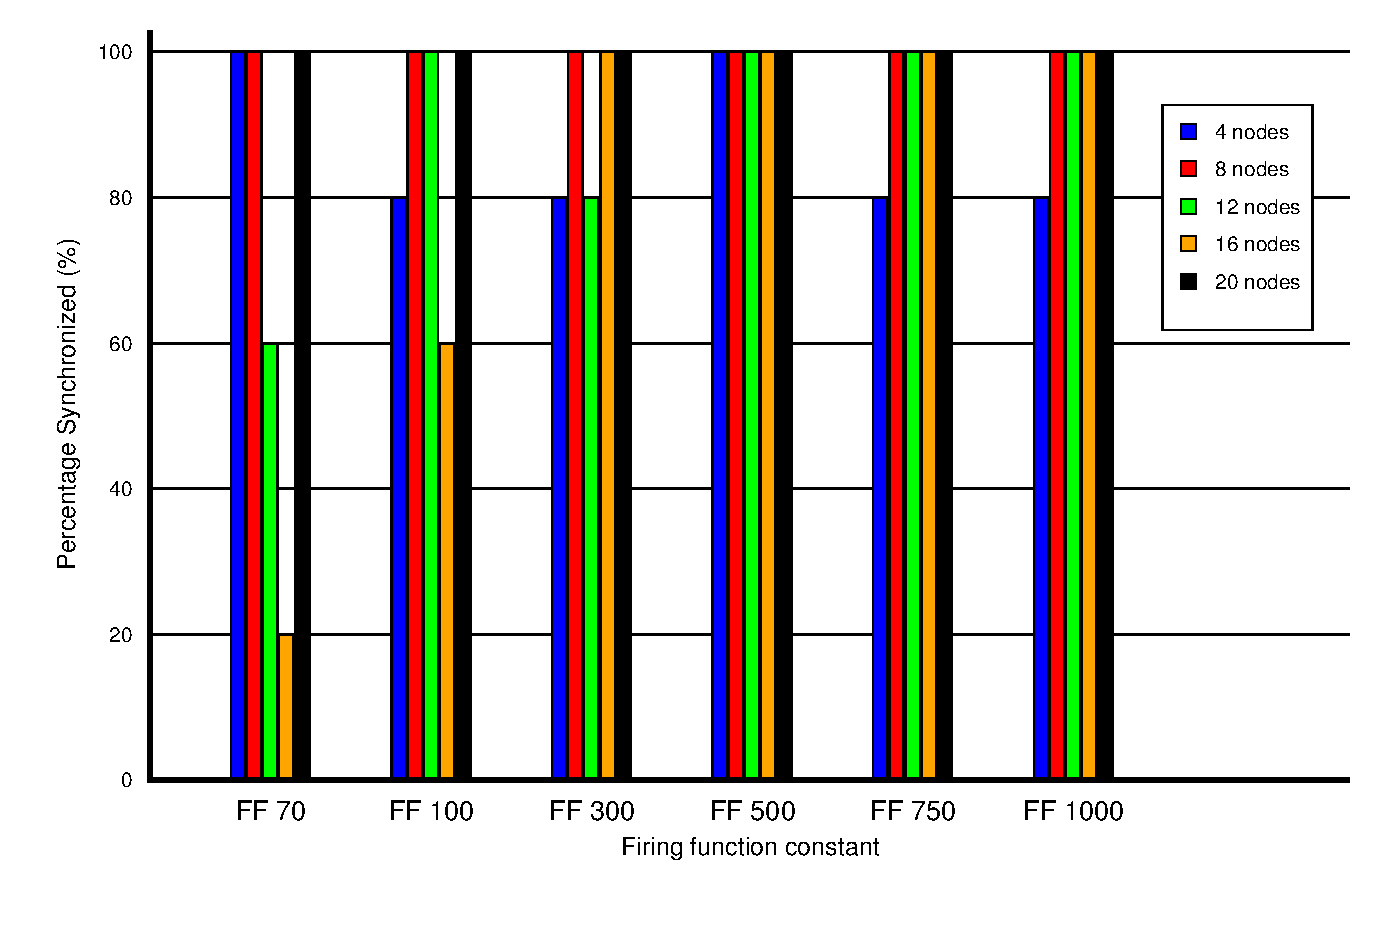
\includegraphics[width=0.4\hsize]{./figures/mdw/ata/percent-synch.pdf}
(b)
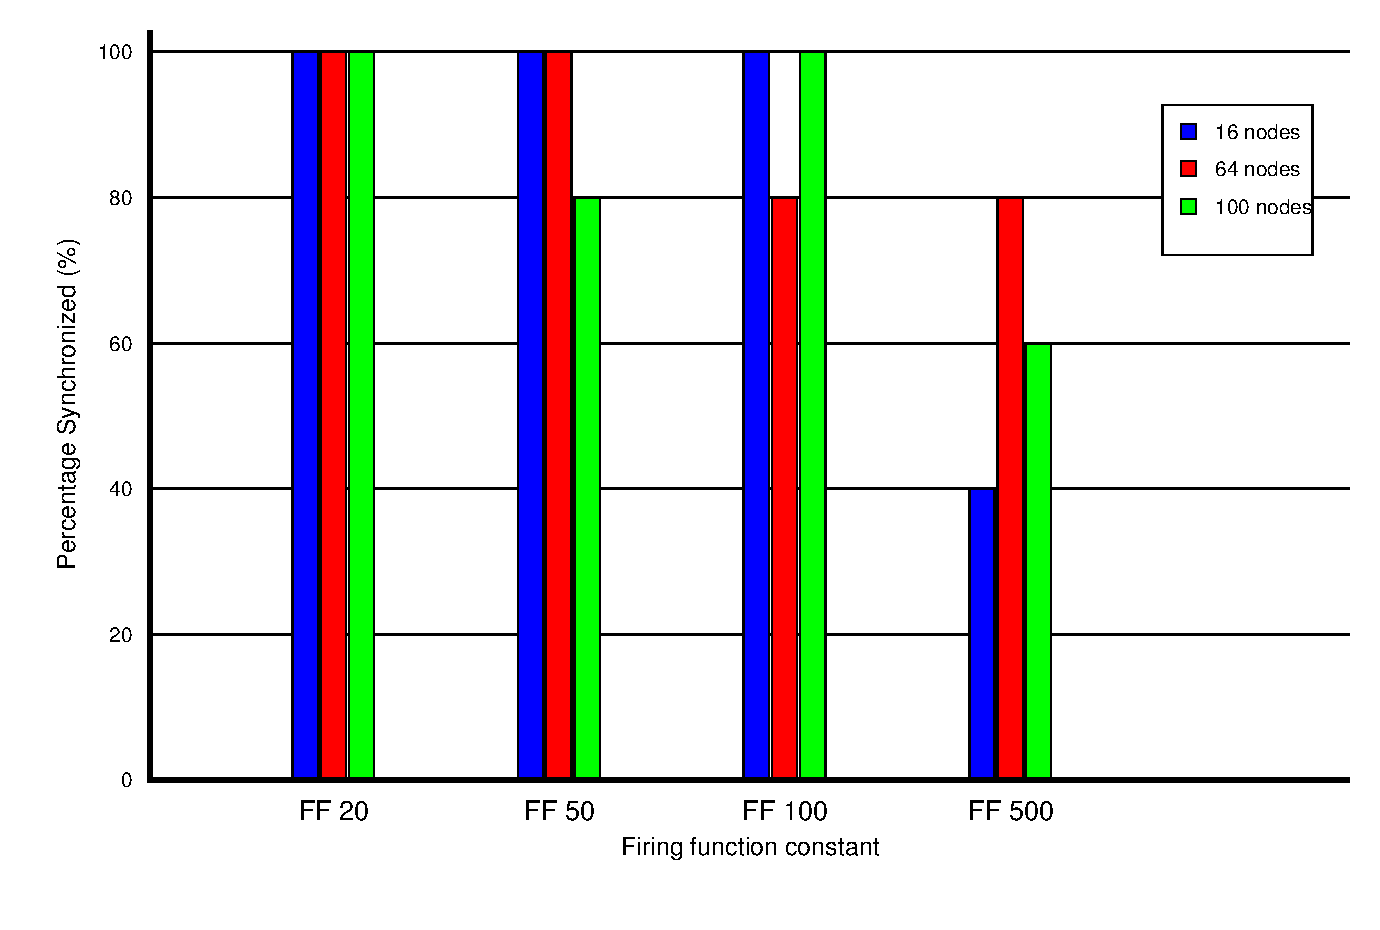
\includegraphics[width=0.4\hsize]{./figures/mdw/grid-synch/percent-synch-grid.pdf}
\end{center}
\caption{Percentage of simulations that achieved synchronicity for
different firing function constants and numbers of nodes. (a)
All-to-all topology. Small firing function constants
(E.g. 10,20,50,150) did not achieve synchronicity most of the
time. (b) Grid Topology. Experiments with very small firing function
constants (E.g. FFC=10) or very large firing function constants
(E.g. $>500$) did not achieve synchronicity.}
\label{fig:pcnt-synch-both}
\end{figure*}

%% all-to-all time to sync and group spread
\begin{figure*}
\centering
(a)
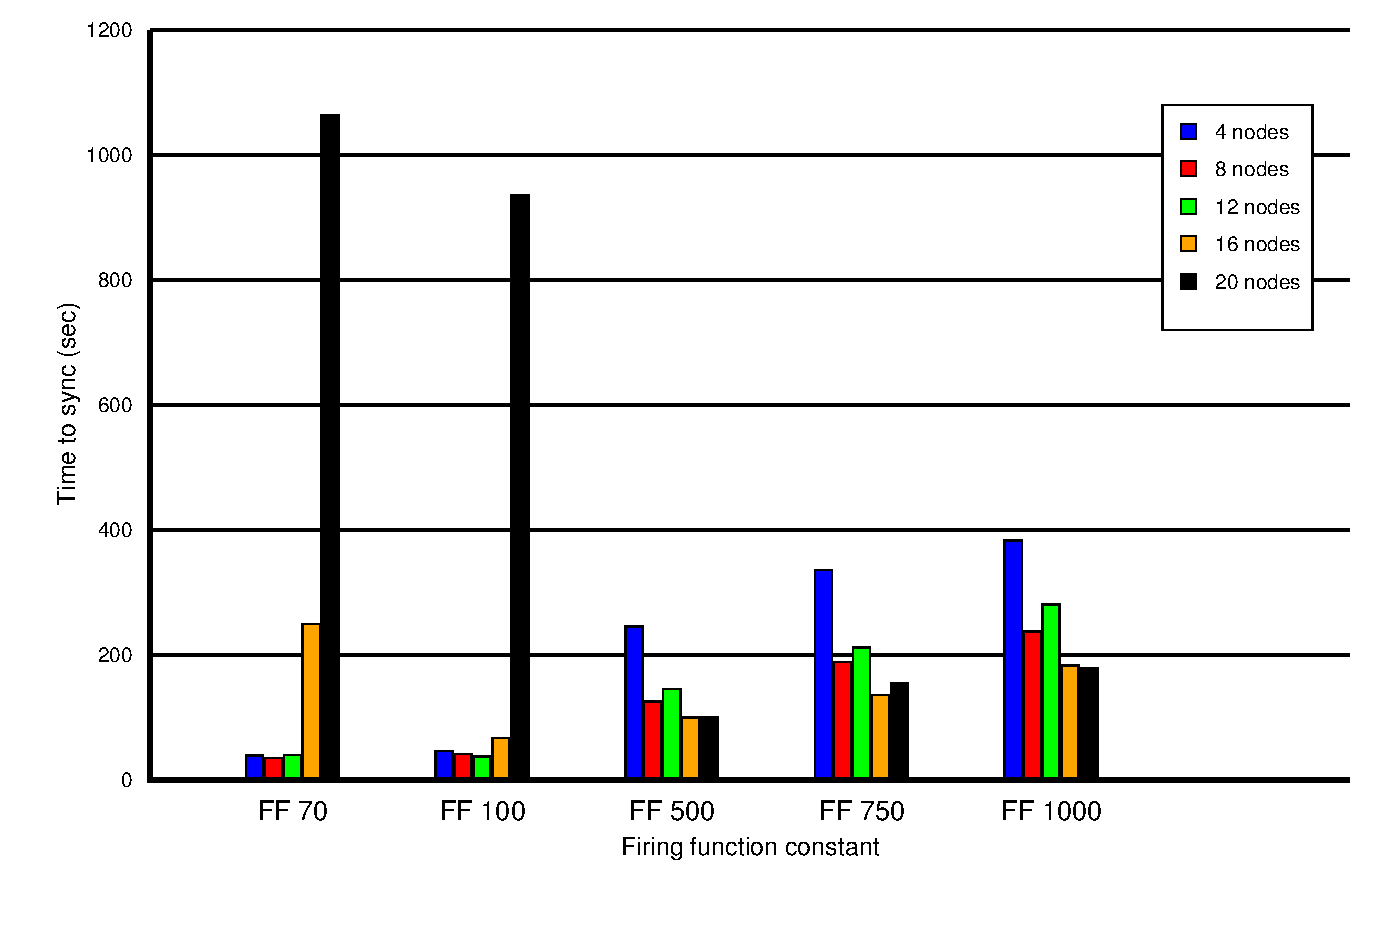
\includegraphics[width=0.4\linewidth]{./figures/mdw/ata/tts.pdf}
(b)
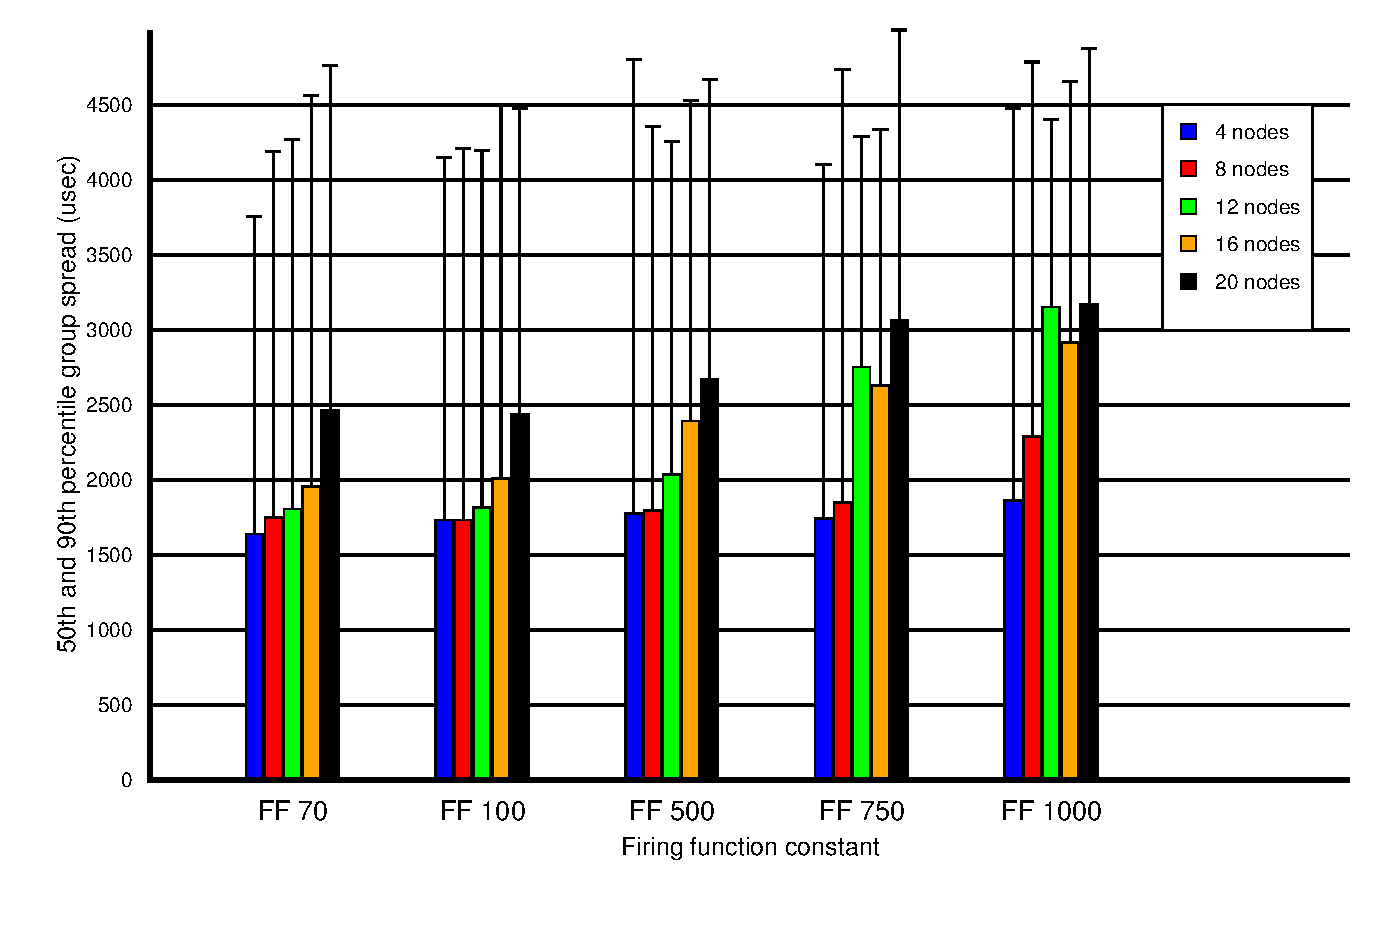
\includegraphics[width=0.4\linewidth]{./figures/mdw/ata/gs-ata.pdf}
\caption{All-to-all topology. (a) Time to Sync, which for most cases
increases with increasing FFC values. (b) Group Spread. The solid bars
represent the 50th percentile spread, while the error bar indicates
the 90th percentile. For most FFC values, the group spreads remain
similar, with a slight increase as the number of nodes increases}
\label{fig:ata}
\end{figure*}

%% grid time to sync and group spread
\begin{figure*}
\begin{center}
(a)
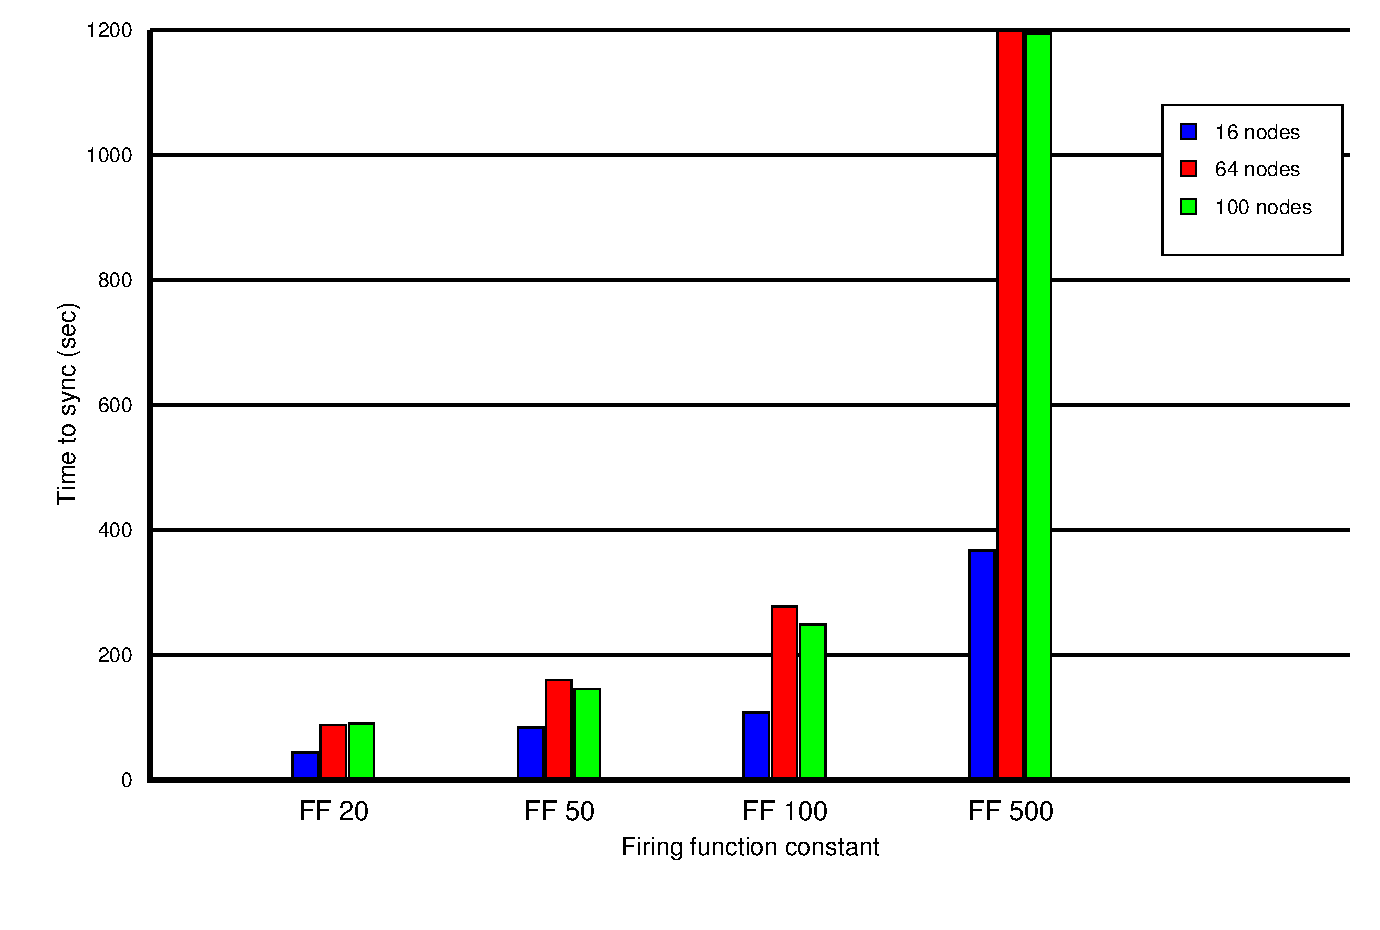
\includegraphics[width=0.4\hsize]{./figures/mdw/grid/tts.pdf}
(b)
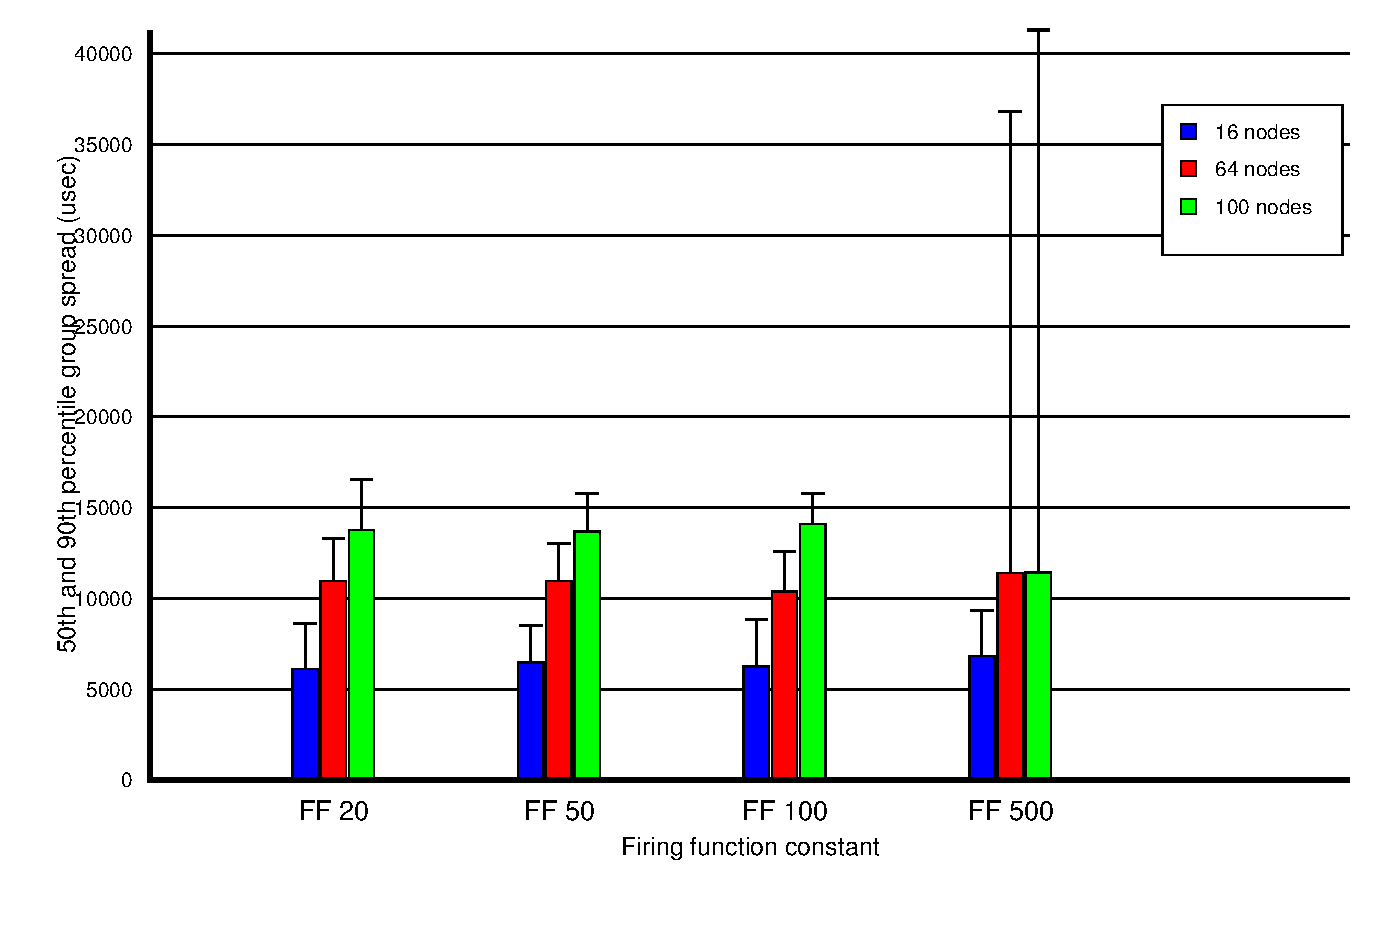
\includegraphics[width=0.4\hsize]{./figures/mdw/grid/gs-grid.pdf}
\end{center}
\caption{Grid Topology. (a) Time to Sync, which increases with
increasing FFC values and network diameter. (b) Group Spread. The
solid bars represent the 50th percentile spread, while the error bar
indicates the 90th percentile. Group spread remains similar over
varying FFC values, but increases with network diameter. For large
grids, FFC=500 does synchronize as well, as also shown in Figure
\ref{fig:pcnt-synch-both}.}
\label{fig:grid}
\end{figure*}

{\bf All-to-all Topology Results.}  Figures
~\ref{fig:pcnt-synch-both}(a) and \ref{fig:ata} show the results of
simulations on the all-to-all topology. We ran simulations for firing
function constant values (FFC) 10,20,50,70,100,150,300,500,750 and
1000, repeating this combination for number of nodes ranging from 2-20
in 2 node increments. For each parameter choice, we ran 10 simulations
using different random seeds to start the nodes at different
times. Each experiment was run for 3600 seconds of simulation
time. Also the time period $T=1$sec for all experiments.

Fig.~\ref{fig:pcnt-synch-both}(a) shows the percentage of simulations
that synchronized for a selection of parameter values. This percentage
represents the fraction of runs that achieved synchronicity out of the
10 total runs, for a given parameter choice of $n$ and $FFC$.  We can
see that the FFC values displayed in the figure (70,100,300,500 and
750) are fairly reliable since these cases achieved synchronicity in a
majority of the simulation runs.  Most experiments with small firing
function constants (10,20,50) did not achieve synchronicity. One
likely reason for this behavior is that small FFC values lead nodes to
make extremely large jumps, causing them to overshoot (see Section
\ref{sec:params}).

Fig.~\ref{fig:ata}(a) shows the time to synchronize as a function of
FFC value and the number of nodes. The graph shows that most FFC
constants work well. The time to sync increases with increasing FFC
value but not beyond 400 time periods. There is no clear trend with
increasing numbers of nodes, although small FFCs do not work as well
with large numbers of nodes. This is possibly because the effect of
overshoot is worsened when there are more neighbors (and thus more
total firing events per cycle to react to).

Fig.~\ref{fig:ata}(b) shows the corresponding group spreads. For most
FFC values and most $n$, the 90th percentile group spread remains the
same. The 50th percentile shows a slight increase with increasing FFCs
and a slight increase with increasing numbers of nodes. However, the
difference in the spreads is not large and thus group spreads remain
fairly similar over all parameter values. The error bars for this data
(not shown here) show that there is not much variation across
different experimental runs.

{\bf Grid Topology Results.}  Fig.~\ref{fig:pcnt-synch-both}(b) and
\ref{fig:grid} show the simulation results for regular grid topologies
of 4x4, 8x8, and 10x10 nodes. Fig. \ref{fig:pcnt-synch-both}(a) shows
the percentage of cases that synchronized for a selection of parameter
values. The results show that FFC values in the range of 20-500 almost
always achieve synchronicity in a grid topology.

The behavior of nodes in a grid topology reflects the impact of
network diameter on performance. Fig.~\ref{fig:grid} (a) shows that
large values of the firing function constant increase the time taken
to achieve synchronicity, and that this effect is more pronounced for
larger grids. Larger FFC values imply that nodes make smaller jumps
and thus converge to synchrony more slowly. For a given FFC, the time
to sync also increases slightly with network diameter, but not by much
for the smaller FFC constants. The error bars for the FFC=500
simulations (not shown here) show that there is a large variation in
time to sync and group spread across runs, most likely caused by the
initial phase distribution of nodes in the grid which can only be
corrected slowly. Barring that case, Fig.~\ref{fig:grid} (b) shows
that the group spread does not vary significantly with FFC
value. However there does seem to be an increase in spread
(i.e. decrease in accuracy) for larger grids, indicating that the
network diameter may have an impact on how well the system can
synchronize.


%%%%%%%%%%%%%%%%%%%%%%%%%%%%%%%%%%%%%%%%%%%%%%%%%%%%%%%%%%%%%%%%%%%%%%%%%%%%%%%%%%%%%%%%%%%%%%%%%%%

%\begin{figure}[p]
%\begin{center}
%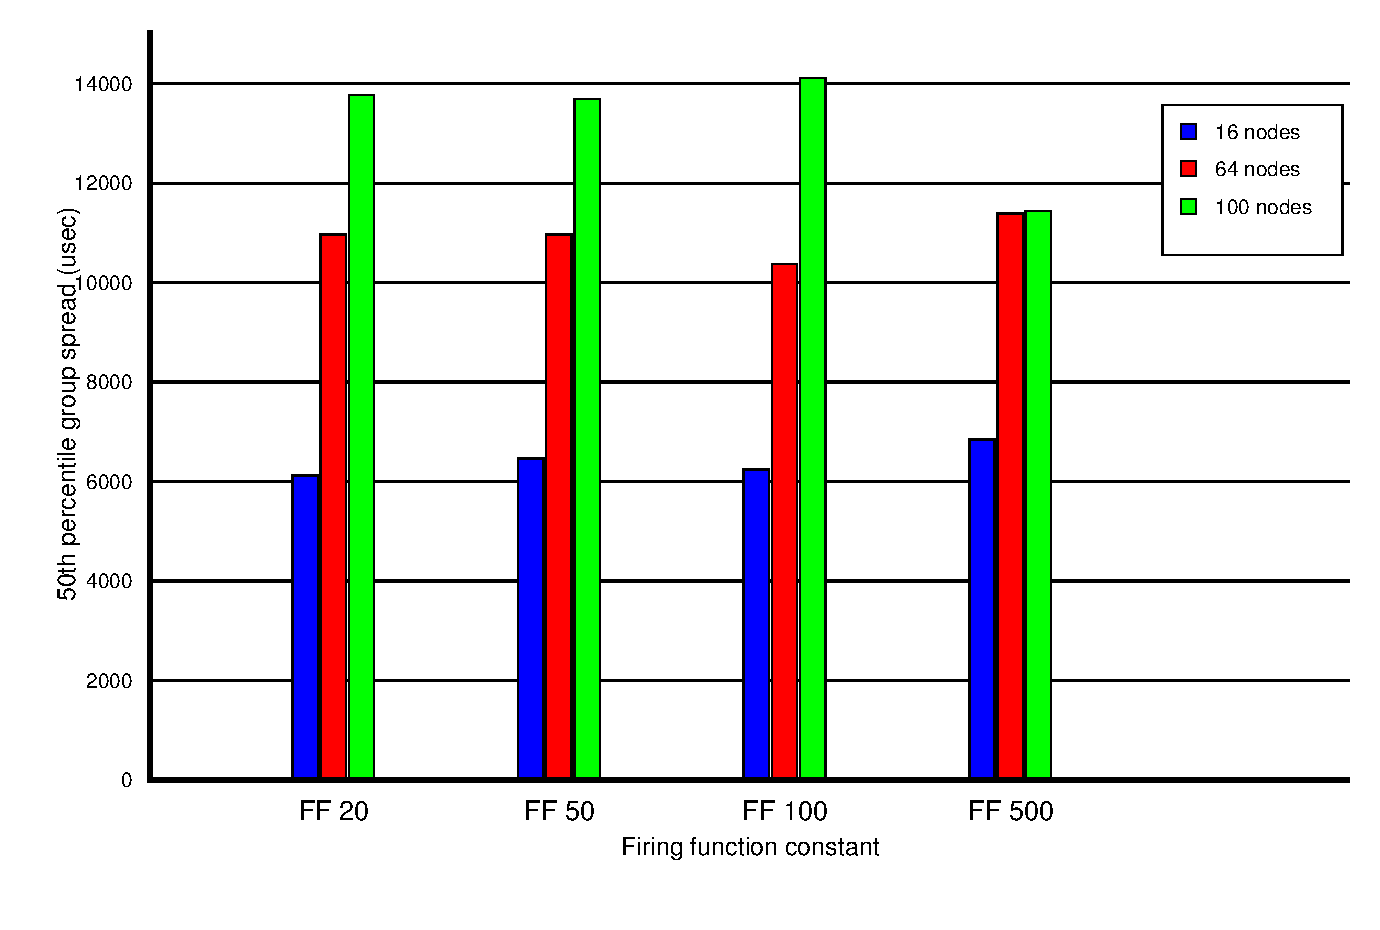
\includegraphics[width=1.0\hsize]{./figures/mdw/grid/gs50.pdf}
%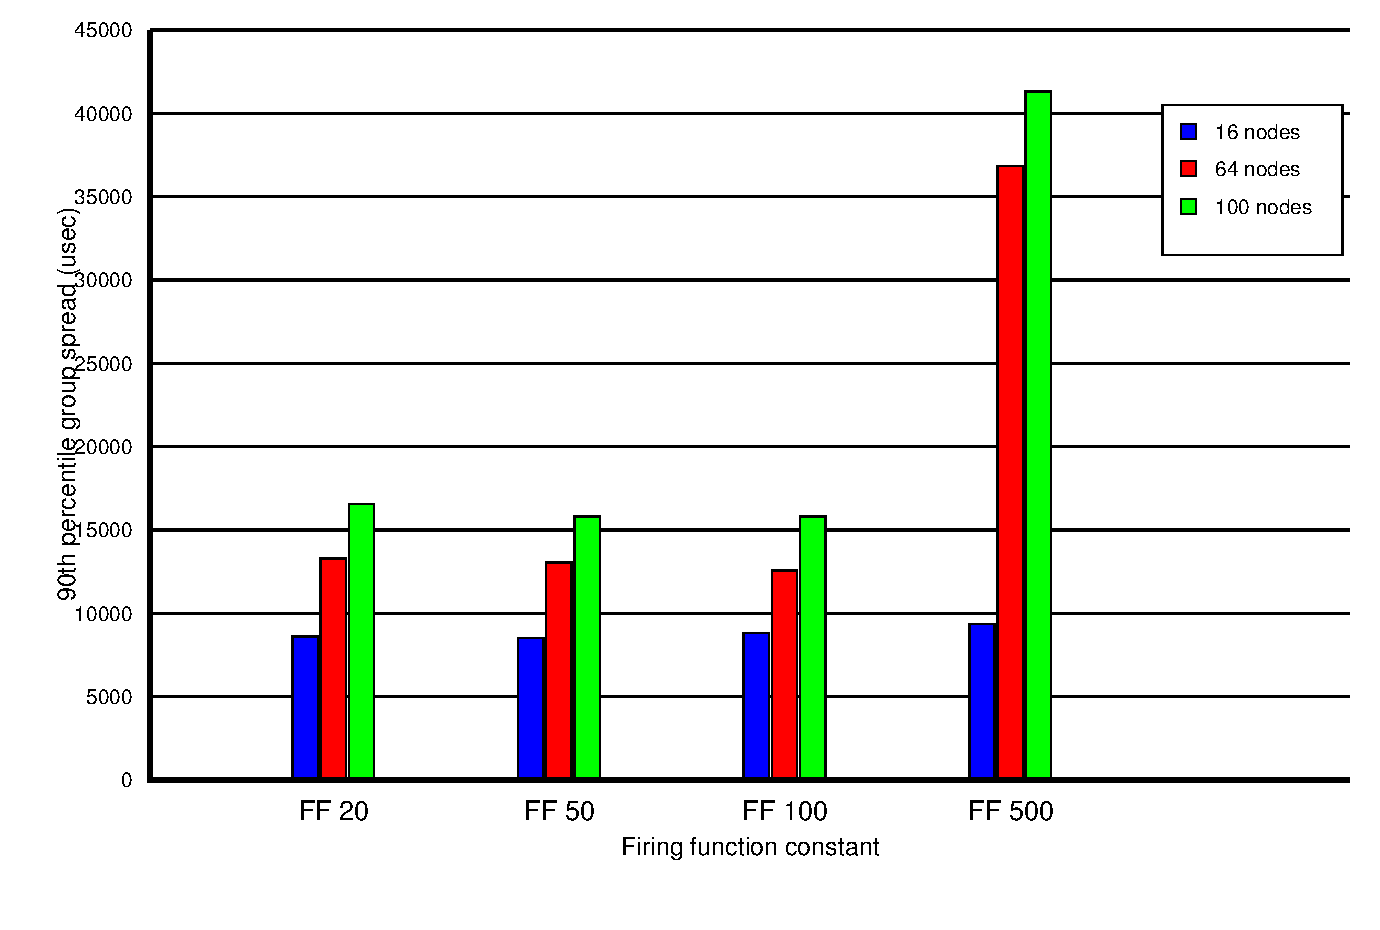
\includegraphics[width=1.0\hsize]{./figures/mdw/grid/gs90.pdf}
%\end{center}
%\caption{{\small {\bf The tightness of the synchronicity decreases with the number of nodes in the grid topology regardless of the number of nodes.  Furthermore, the firing function constant does not have a significant impact on the tightness of synchronicity in this topology.  These trends are retained in the 90th percentile group spread.}}}
%\label{fig:grid90}
%\end{figure}

%\begin{figure}[p]
%\begin{center}
%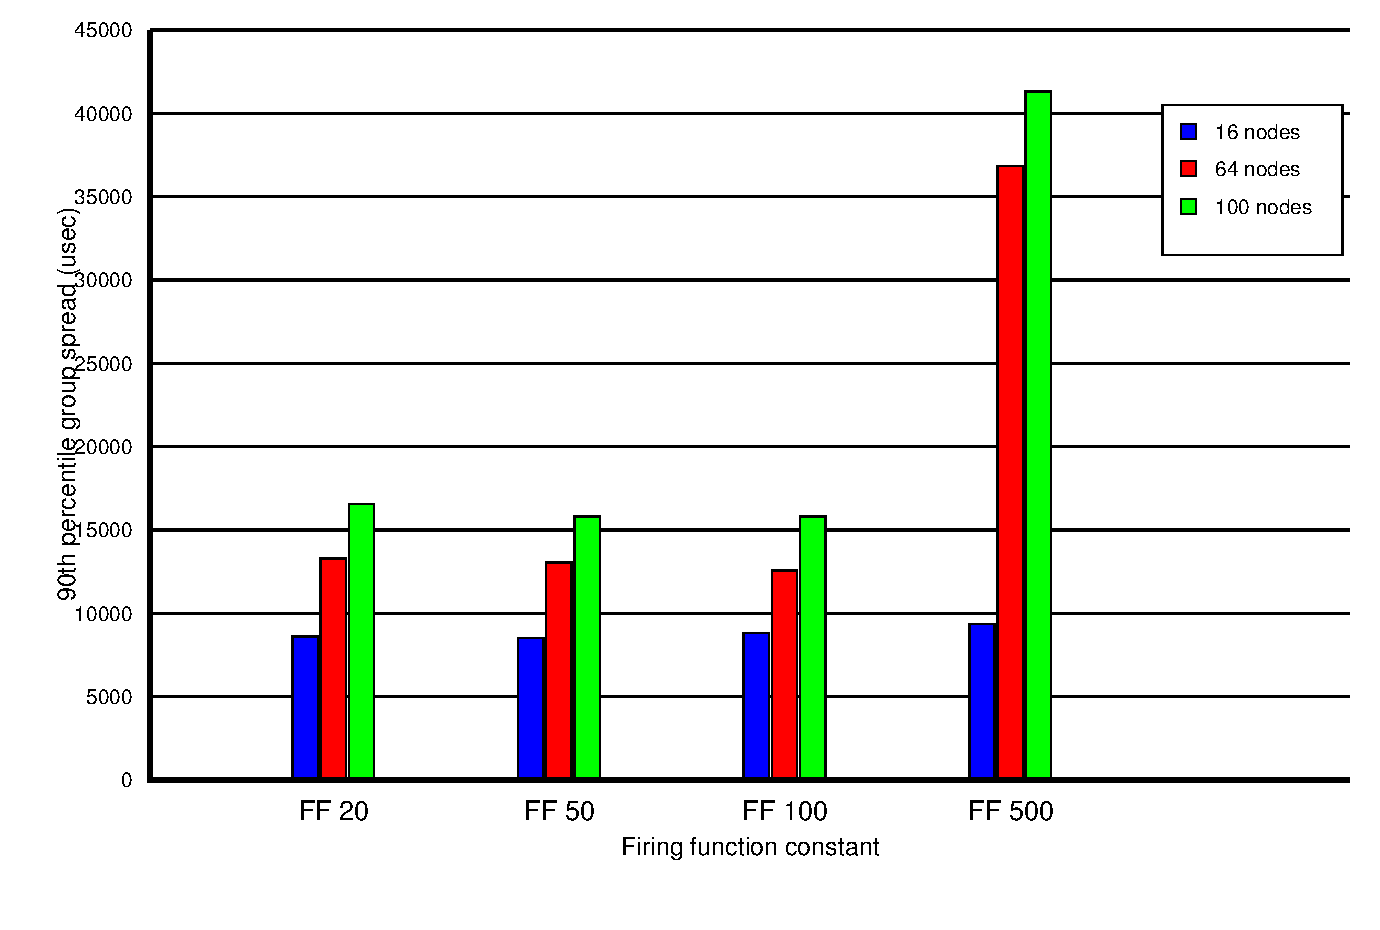
\includegraphics[width=1.0\hsize]{./figures/mdw/grid/gs90.pdf}
%\end{center}
%\caption{{\small {\bf 90th percentile group spread in the grid topology for different number of nodes}}}
%\label{fig:grid90}
%\end{figure}

%\begin{table}[t]
%\begin{center}
%\begin{tabular}{|c|c|c|} \hline
%Topology & Number of Nodes & Firing Function Constant \\ \hline \hline
%%all-to-all &  2  &  1000 \\
%all-to-all &  6  &  10 \\
%all-to-all &  8  &  20 \\ 
%all-to-all &  10 &  10 \\
%all-to-all &  10 &  20 \\
%all-to-all &  12 &  20 \\
%all-to-all &  12 &  50 \\
%all-to-all &  14 &  10 \\
%all-to-all &  14 &  20 \\ 
%all-to-all &  14 &  50 \\
%all-to-all &  16 &  20 \\
%all-to-all &  18 &  20 \\
%all-to-all &  20 &  20 \\ 
%grid       &  64 &  10 \\
%grid       &  64 &  750 \\
%grid       &  64 &  1000 \\
%grid       &  100 &  750 \\
%grid       &  100 &  1000 \\ \hline \hline
%\end{tabular}
%\end{center}
%\caption{{\small Cases that did not achieve synchronicity consistently across all experimental runs.}}
%\label{table:nosync}
%\end{table}

%Table ~\ref{table:nosync} shows that this occurred particularly for a firing function constant value of 20.
%As explained in section 3.4, theoretical analysis predicts that the smaller the firing function
%constant value (i.e. large $\epsilon$), the larger a node jumps in response to other nodes,
%and thus nodes should converge to synchrony faster. 


%\begin{figure}[p]
%\begin{center}
%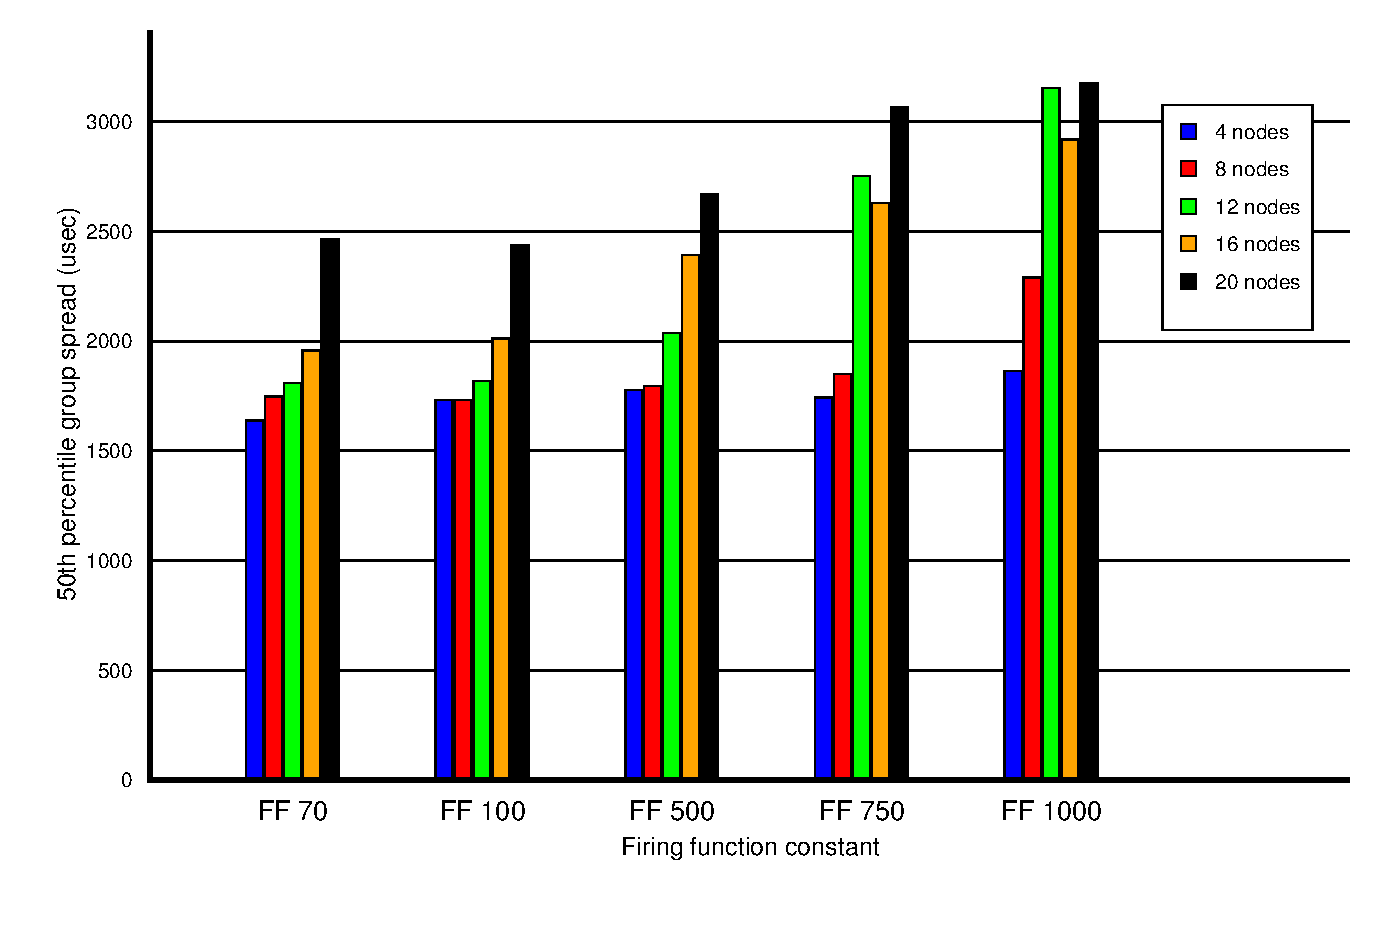
\includegraphics[width=0.9\linewidth]{./figures/mdw/ata/gs50.pdf}
%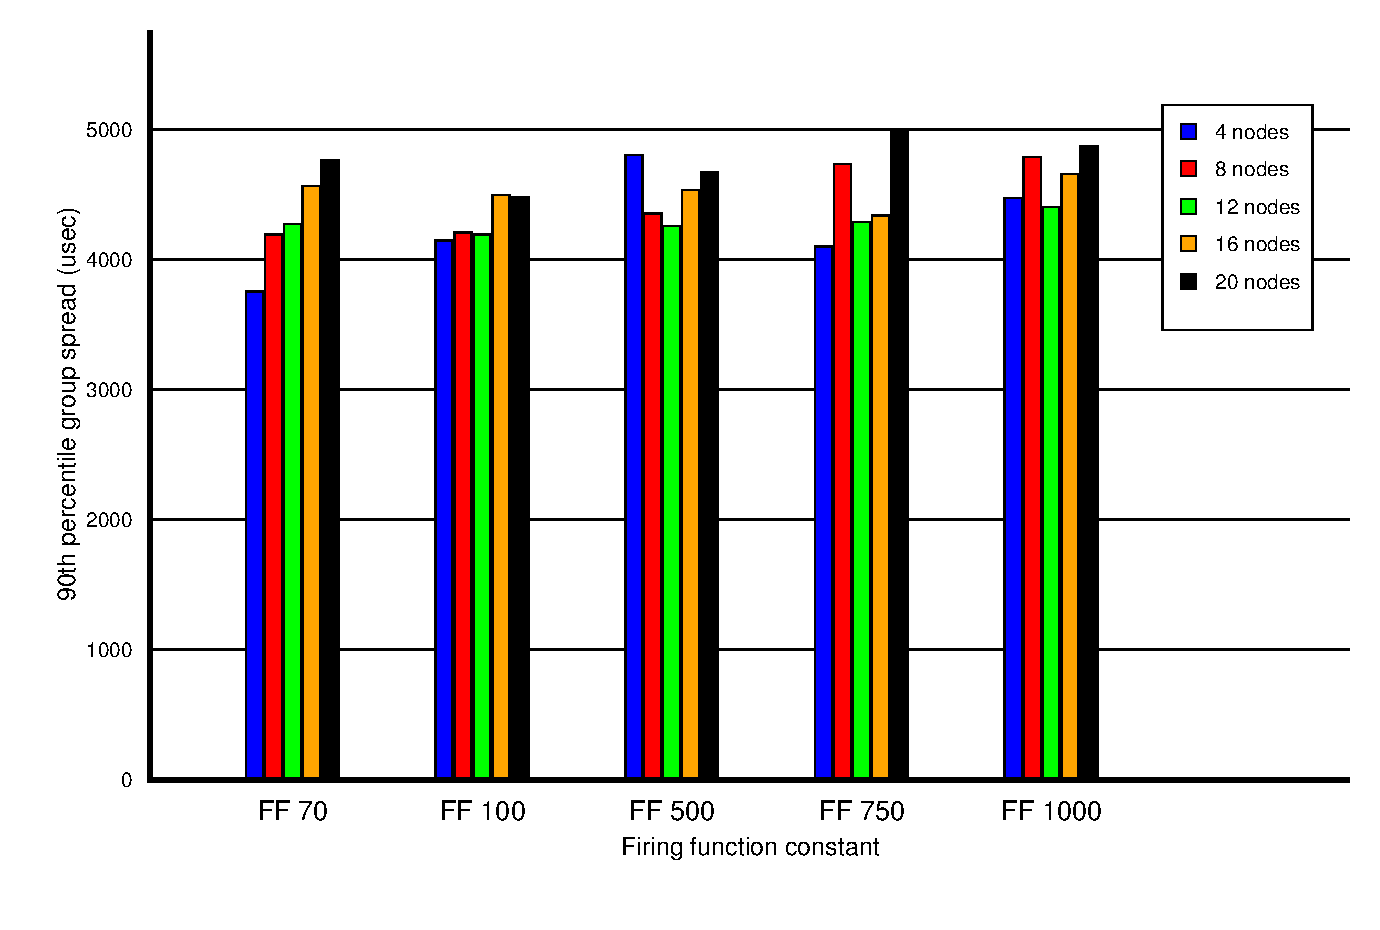
\includegraphics[width=1.0\hsize]{./figures/mdw/ata/gs90.pdf}
%\end{center}
%\caption{{\small {\bf The tightness of synchronicity for half of the groups does not vary dramatically across different firing function constant values, but does increase with the number of nodes in an all-to-all topology.  The magnitude of the increase however is quite small.}}}
%\label{fig:ata50}
%\end{figure}

%\begin{figure}[p]
%\begin{center}
%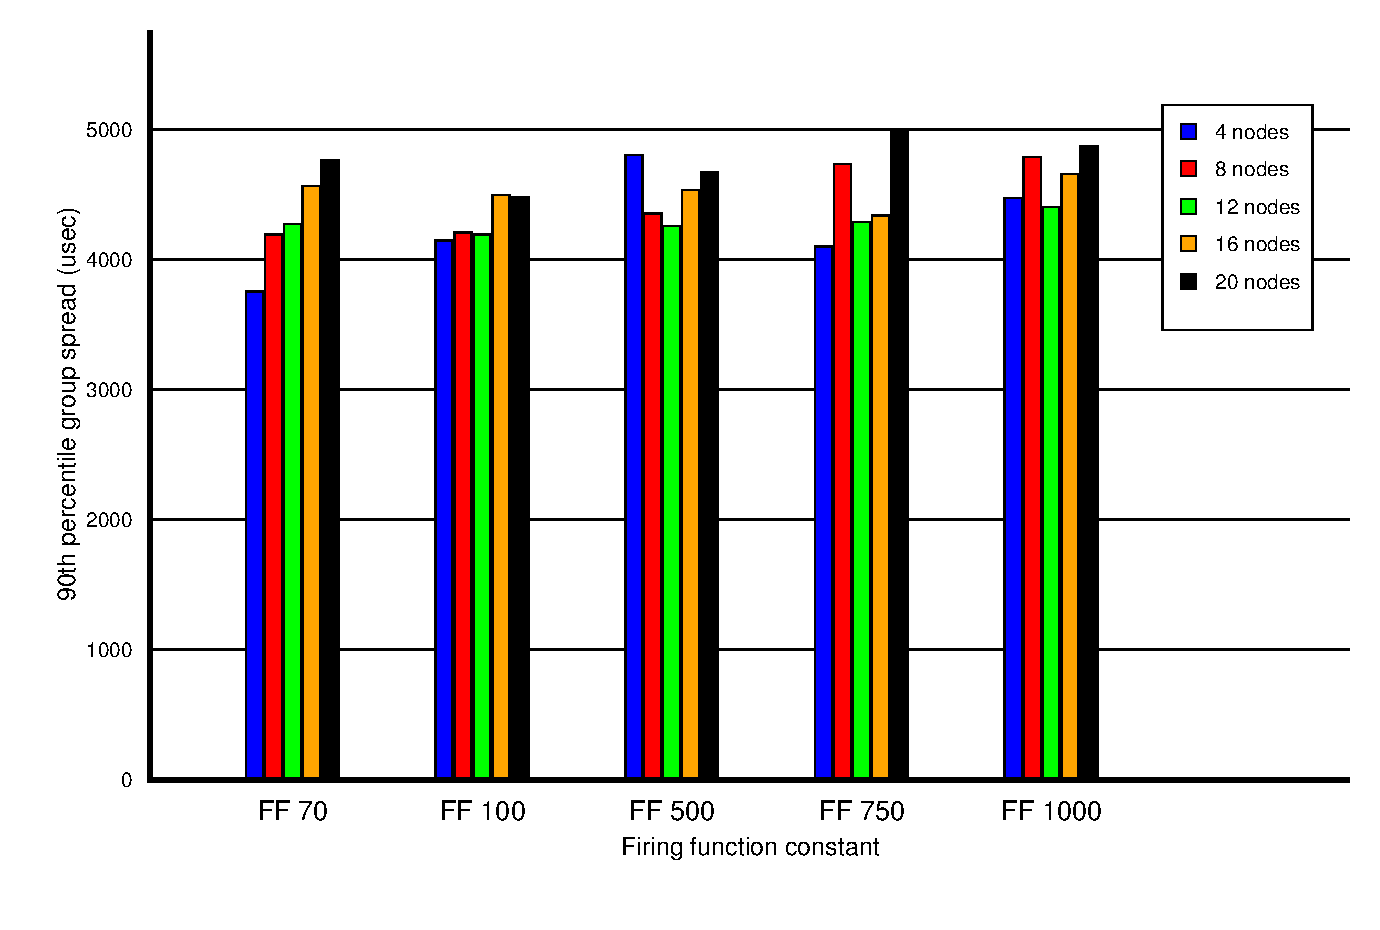
\includegraphics[width=1.0\hsize]{./figures/mdw/ata/gs90.pdf}
%\end{center}
%%\caption{{\small {\bf 90th percentile group spread for different number of nodes in the all-to-all topology}}}
%\label{fig:ata90}
%\end{figure}



%%% OLD FIGURES %%%%

%% \begin{figure*}
%% \begin{center}
%% (a)
%% 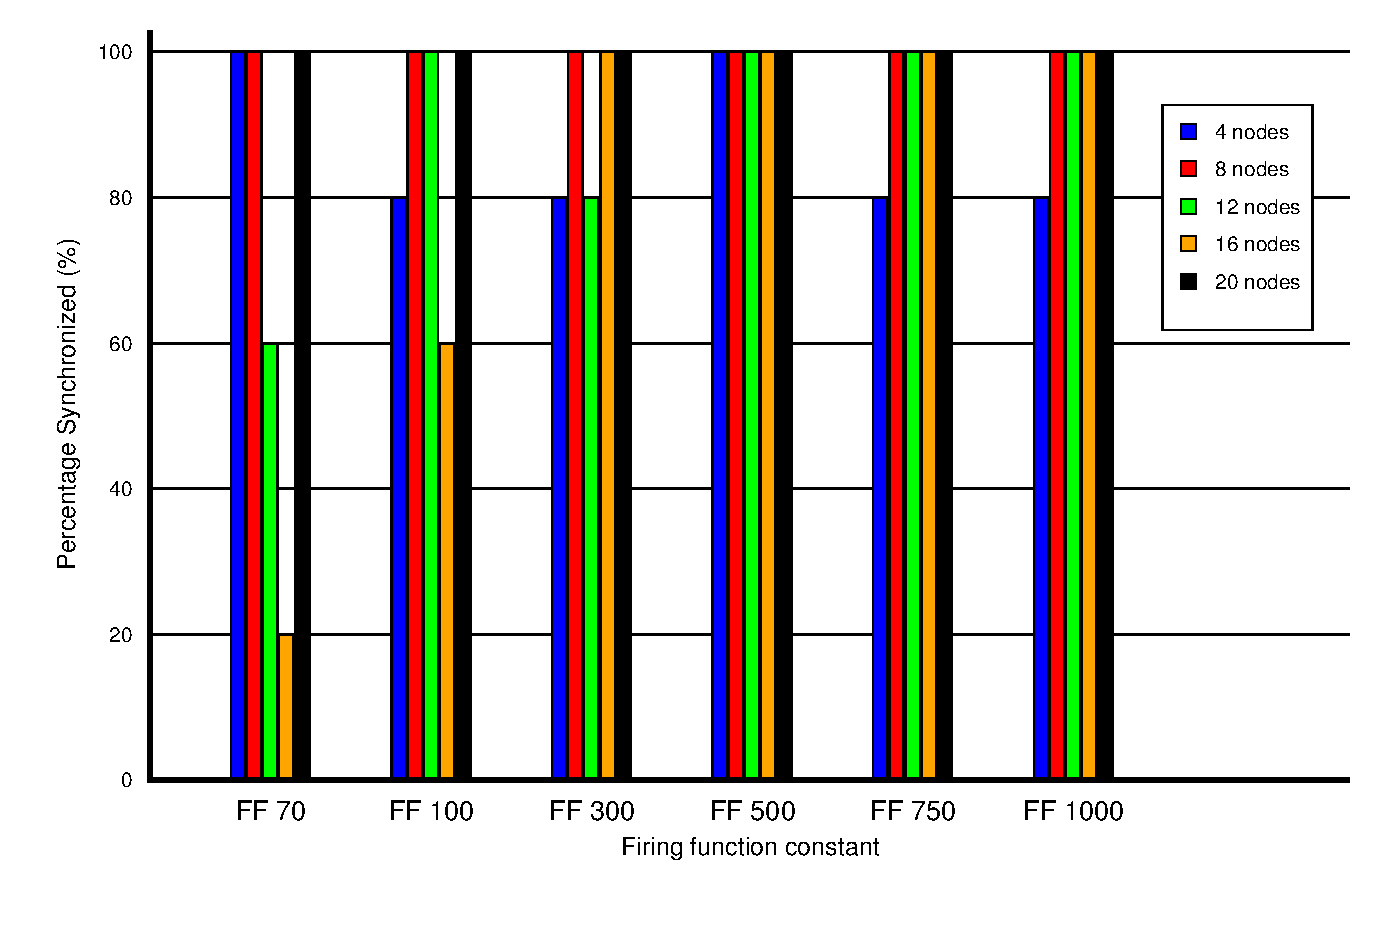
\includegraphics[width=0.4\hsize]{./figures/mdw/ata/percent-synch.pdf}
%% (b)
%% 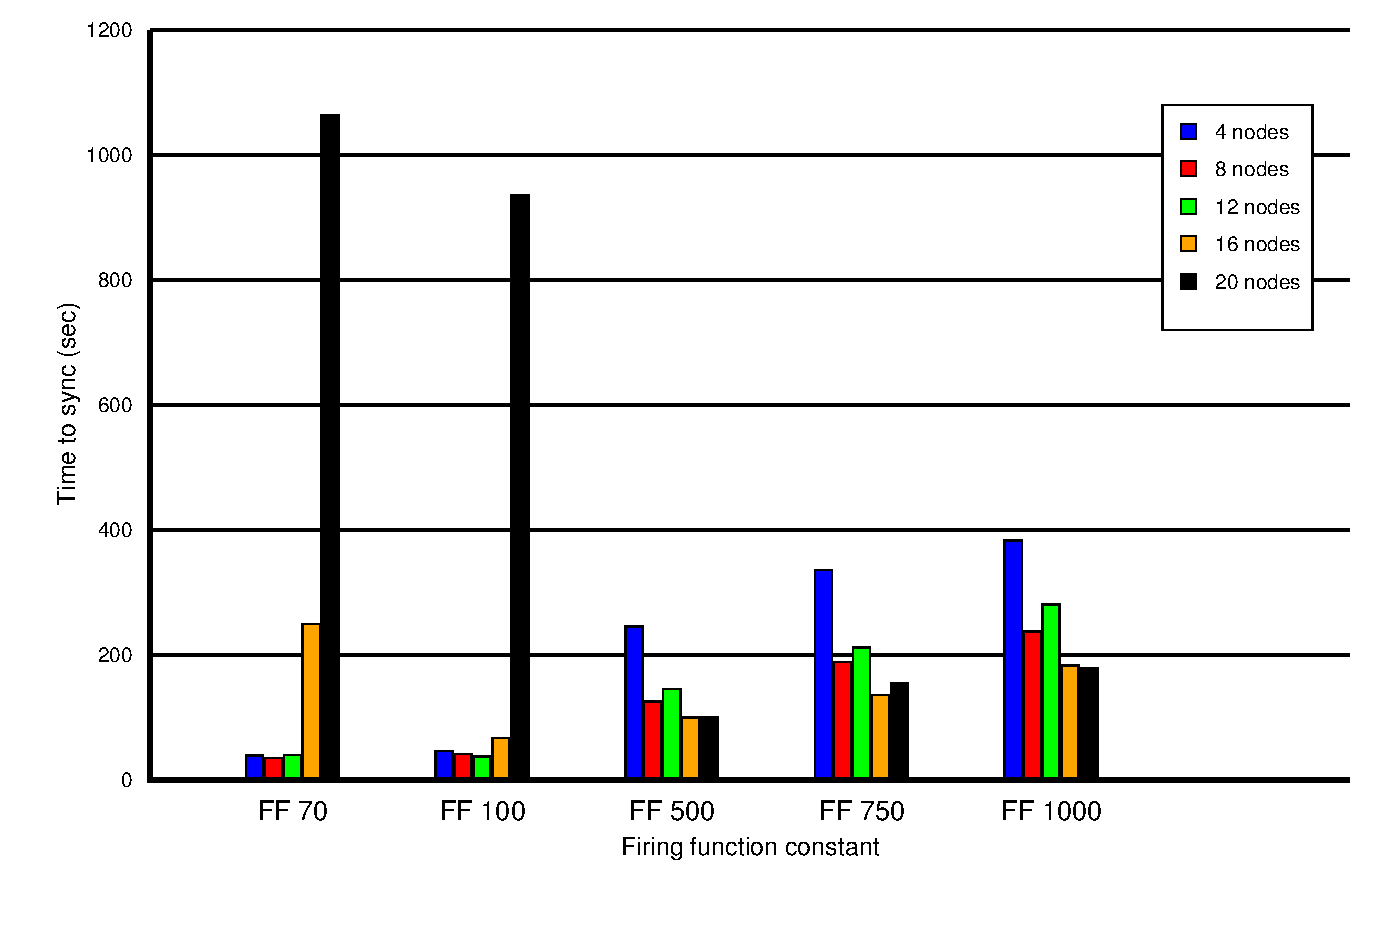
\includegraphics[width=0.4\hsize]{./figures/mdw/ata/tts.pdf}
%% \end{center}
%% \caption{All-to-all topology: (a) Percentage of simulations that
%% achieved synchronicity for different firing function constants and
%% numbers of nodes. Small firing function constants (E.g. 10,20,50,150)
%% did not achieve synchronicity most of the time. (b) For most cases,
%% the time to sync was similar over large range of FFCs.}
%% \label{fig:pcnt-synch-ata}
%% \end{figure*}

%% %% \label{fig:alltts}


%% \begin{figure*}
%% \centering
%% (a)
%% 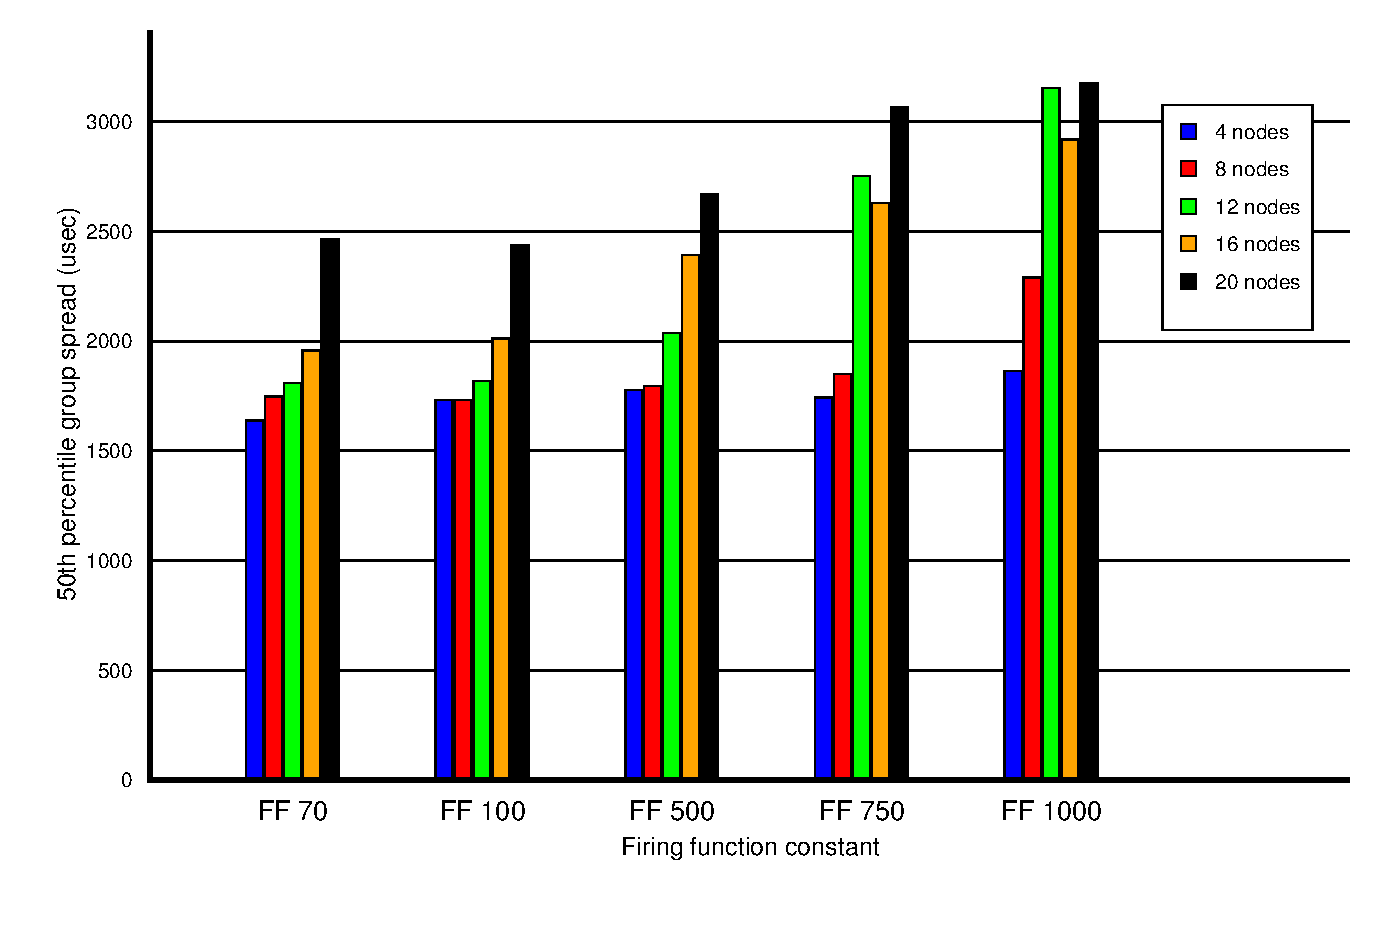
\includegraphics[width=0.4\linewidth]{./figures/mdw/ata/gs50.pdf}
%% (b)
%% 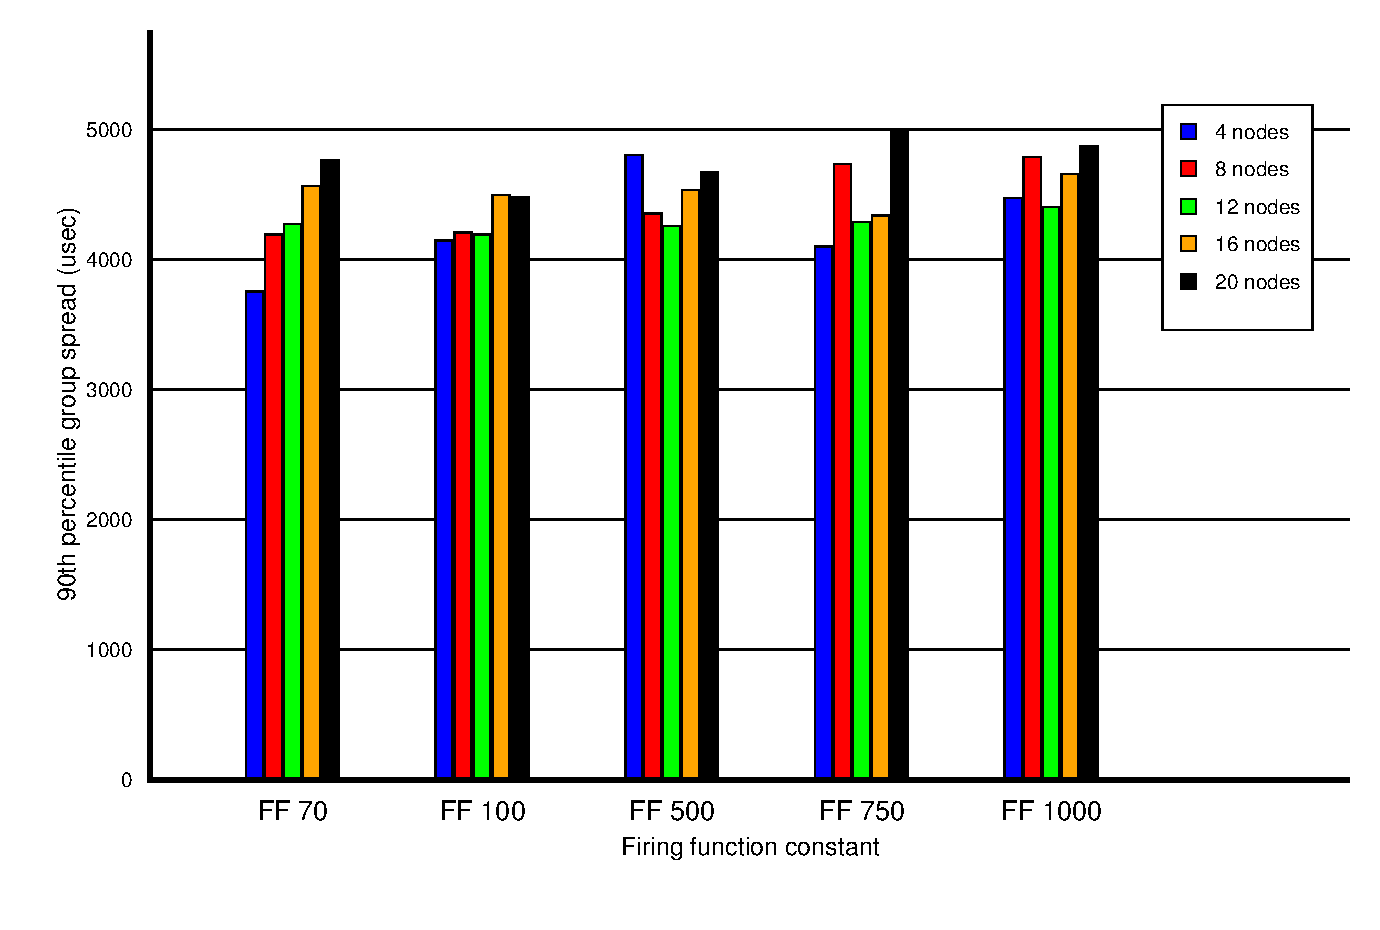
\includegraphics[width=0.4\linewidth]{./figures/mdw/ata/gs90.pdf}
%% \caption{All-to-all topology: The tightness of synchronicity for the
%% groups does not vary dramatically across different firing function
%% constant values or with different number of nodes.}
%% \label{fig:ata-gs}
%% \end{figure*}

%% %% \subfigure[]
%% %%   {\framebox{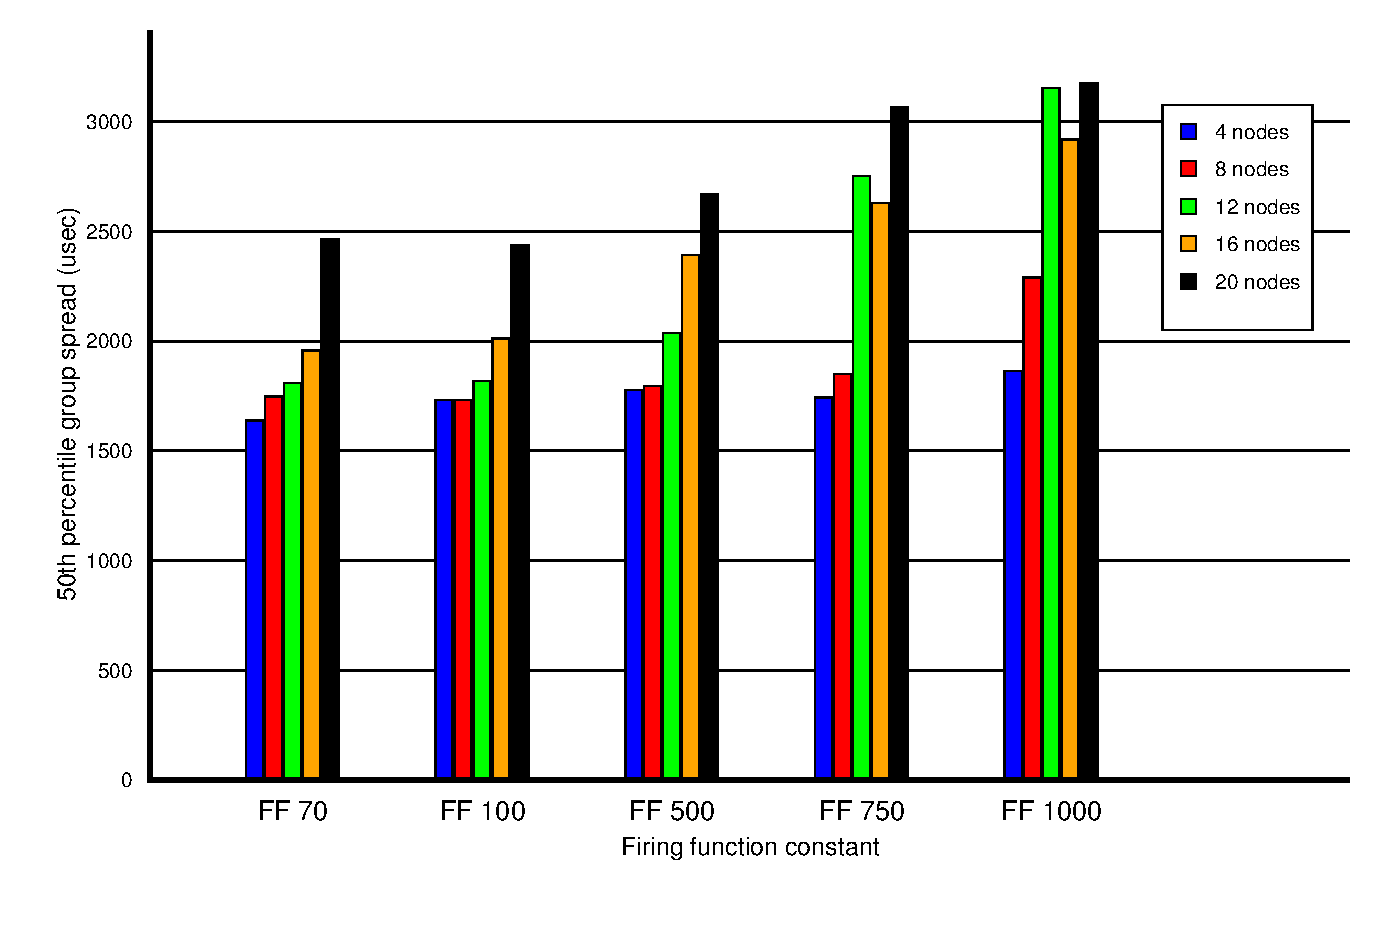
\includegraphics[width=0.4\linewidth]{./figures/mdw/ata/gs50.pdf}}}
%% %% \quad\quad
%% %% \subfigure[]
%% %%   {\framebox{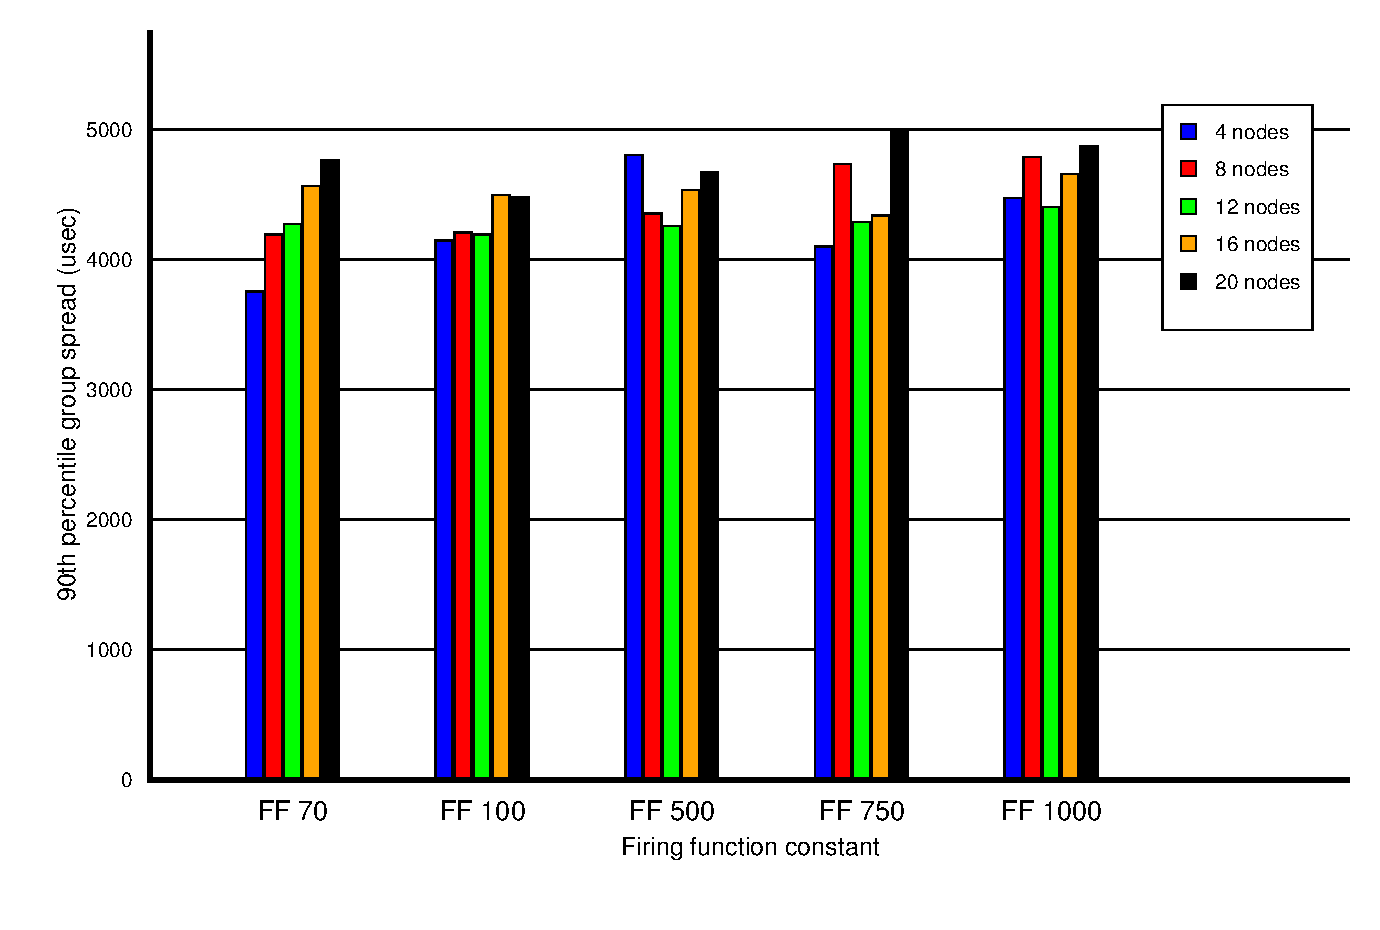
\includegraphics[width=0.4\linewidth]{./figures/mdw/ata/gs90.pdf}}}

%% \begin{figure*}
%% \begin{center}
%% (a)
%% 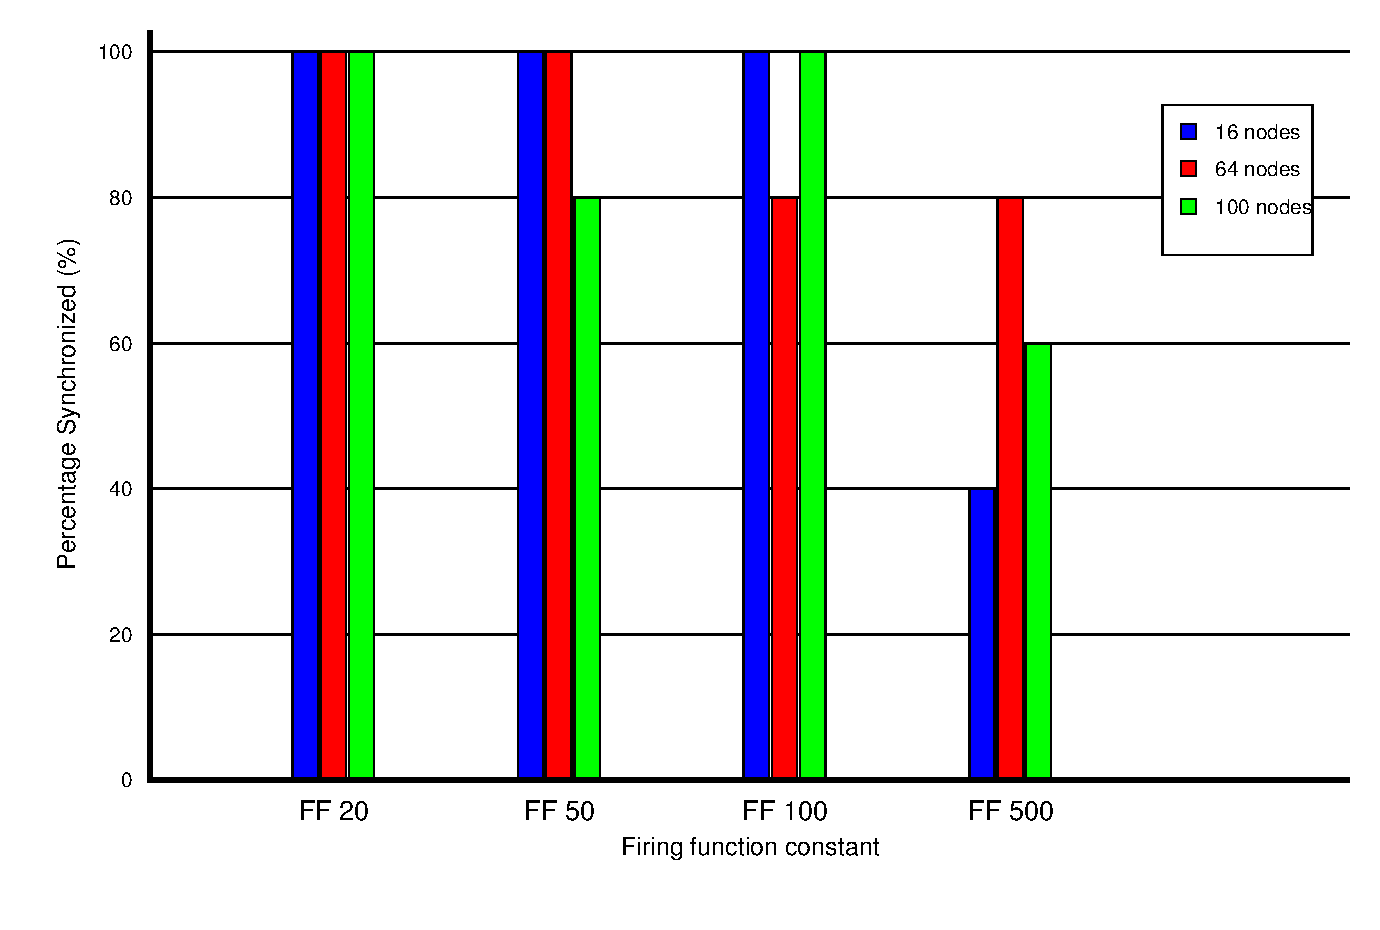
\includegraphics[width=0.4\hsize]{./figures/mdw/grid-synch/percent-synch-grid.pdf}
%% (b)
%% 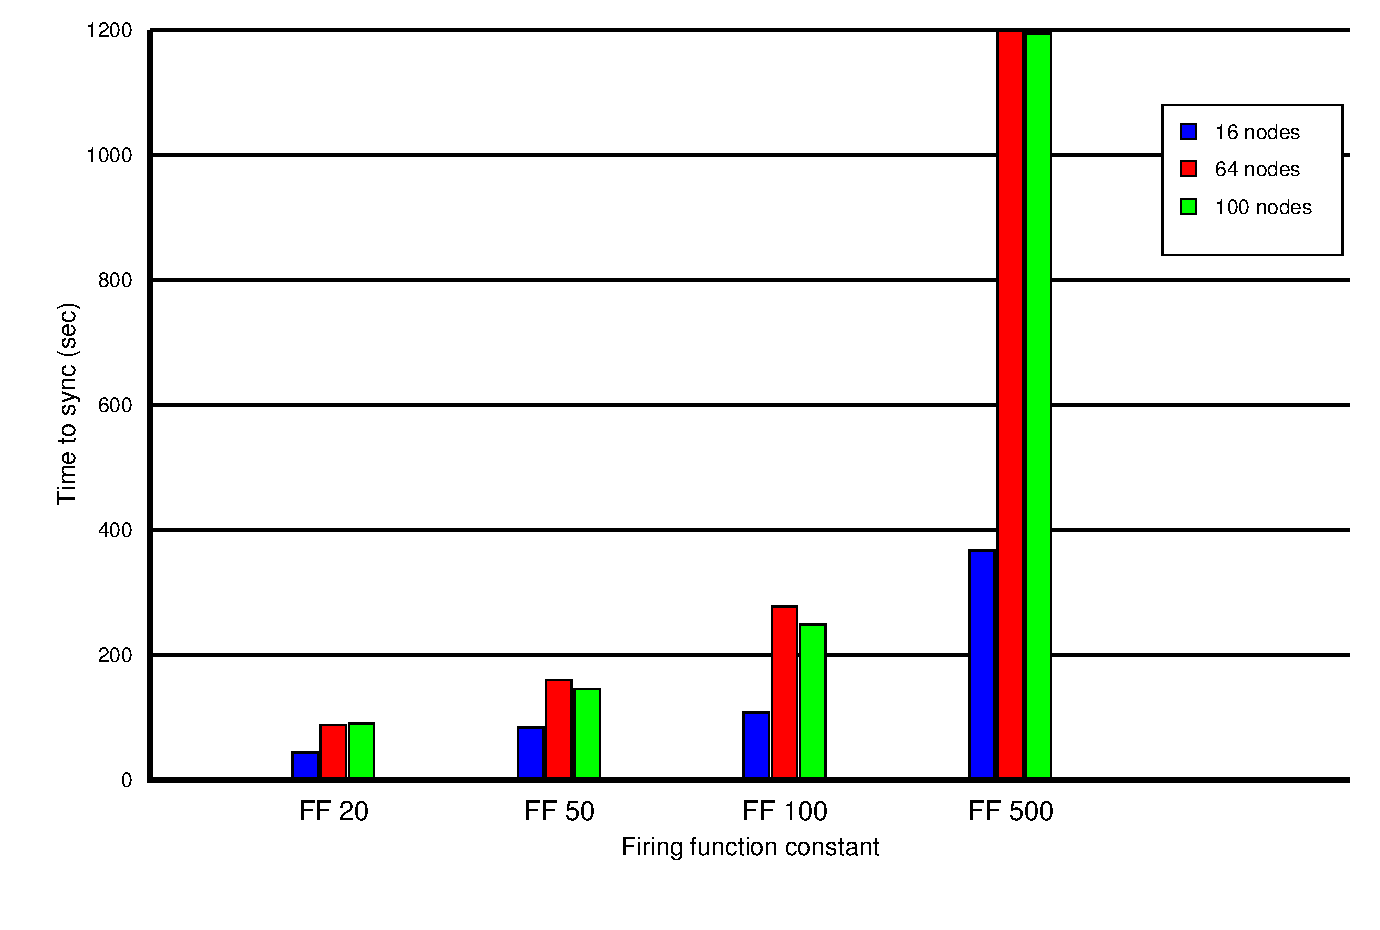
\includegraphics[width=0.4\hsize]{./figures/mdw/grid/tts.pdf}
%% \end{center}
%% \caption{Grid Topology: (a) Experiments involving very small firing
%% function constants (E.g. FFC=10) or very large firing function
%% constants (E.g. $>500$) did not achieve synchronicity. (b) The
%% relationship between FFC and the time to synch follows the theoretical
%% predictions near-perfectly in a grid topology.}
%% \label{fig:pcnt-synch-grid}
%% \end{figure*}

%% %\label{fig:grid-tts}
%% %\end{figure}

%% \begin{figure*}
%% \centering
%% (a)
%% 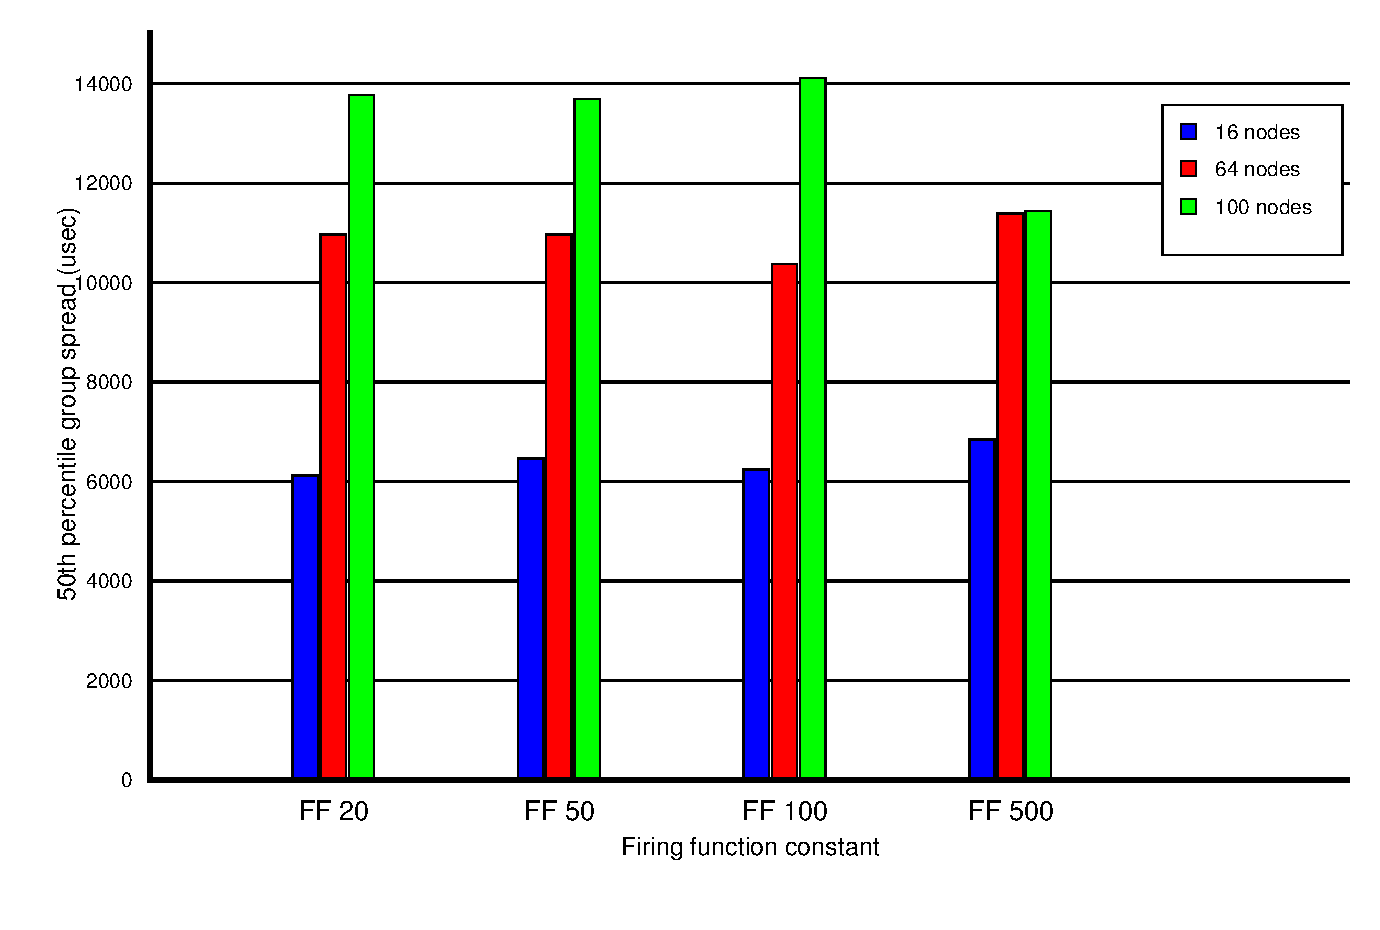
\includegraphics[width=0.4\linewidth]{./figures/mdw/grid/gs50.pdf}
%% (b)
%% 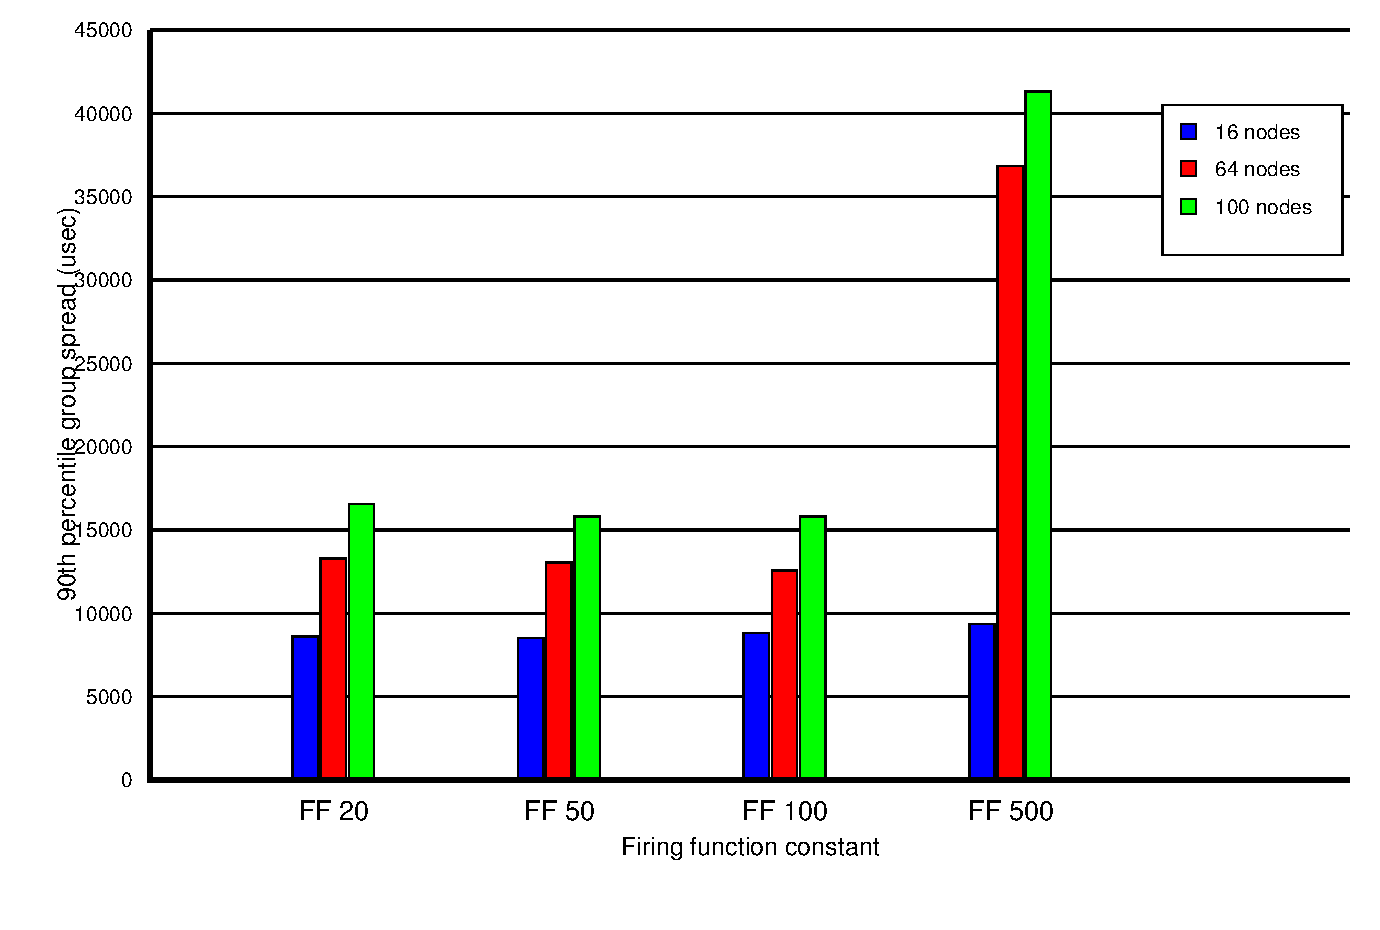
\includegraphics[width=0.4\linewidth]{./figures/mdw/grid/gs90.pdf}
%% \caption{Grid Topology: The tightness of synchronicity decreases with
%% the number of nodes in the grid topology, while the FFC does not have
%% a sginificant impact.}
%% \label{fig:grid-gs}
%% \end{figure*}

%% %% \subfigure[]
%% %%   {\framebox{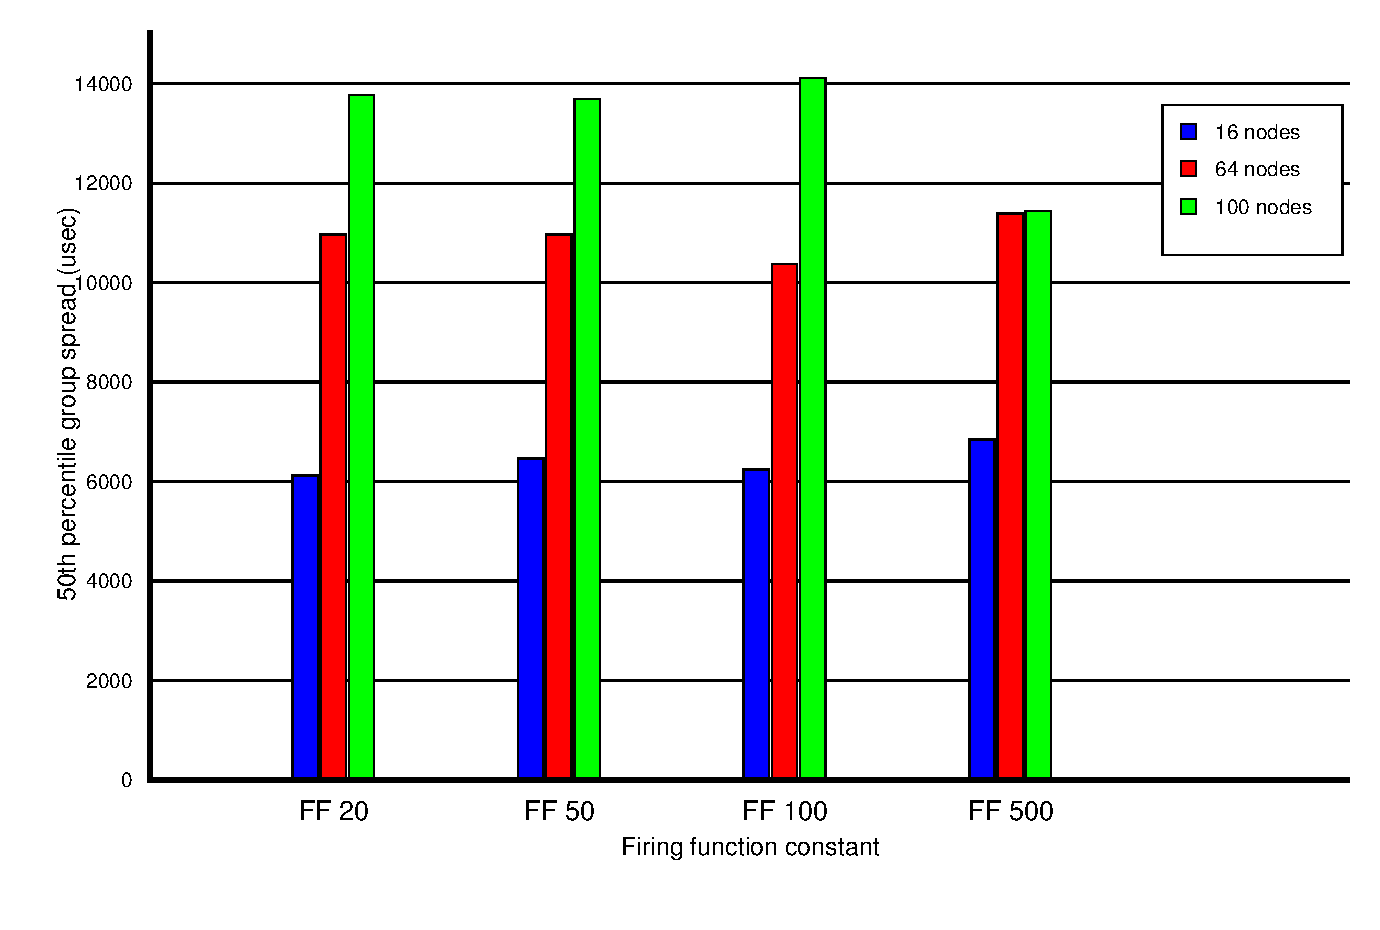
\includegraphics[width=0.4\linewidth]{./figures/mdw/grid/gs50.pdf}}}
%% %% \quad\quad
%% %% \subfigure[]
%% %%   {\framebox{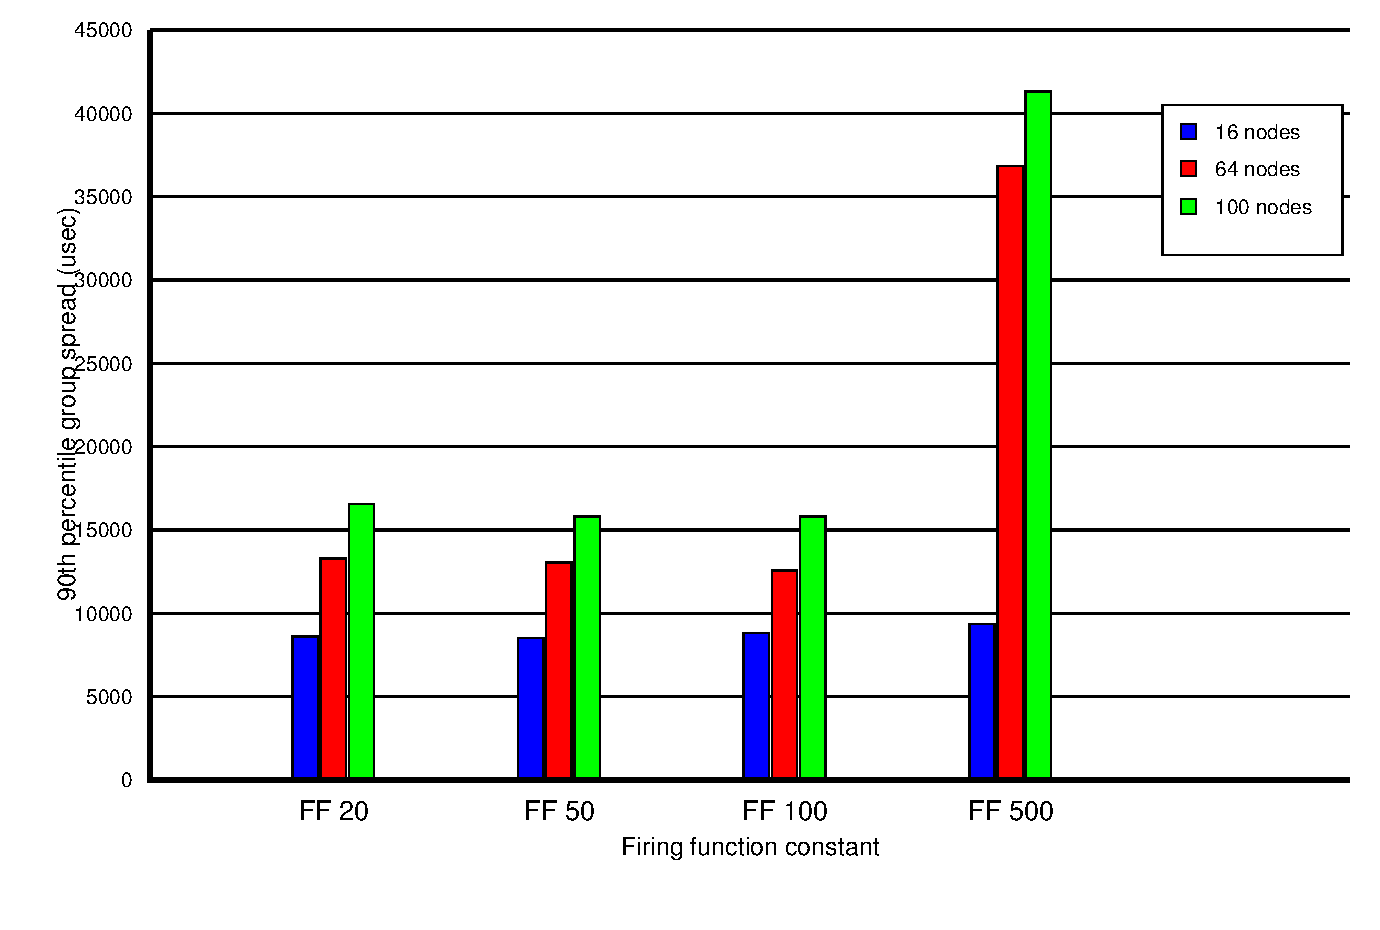
\includegraphics[width=0.4\linewidth]{./figures/mdw/grid/gs90.pdf}}}


